\documentclass[10pt,letterpaper]{article}

\usepackage{epsfig}
\usepackage{graphicx}
\usepackage{amsmath}
\usepackage{algorithm}
\usepackage{algorithmic}
\usepackage{amssymb}
\usepackage{amsthm}
\usepackage{cmap}
\usepackage[a4paper]{geometry}

\usepackage[pagebackref=true,breaklinks=true,letterpaper=true,colorlinks,bookmarks=false]{hyperref}

\newcommand{\comment}[1]{}
\newcommand{\floor}[1]{\lfloor #1 \rfloor}
\newcommand{\argmin}{\operatornamewithlimits{argmin}}
\newcommand{\argmax}{\operatornamewithlimits{argmax}}

\newcommand{\mysection}[1]{\vspace{0mm}\section{#1}\vspace{0mm}}
\newcommand{\mysubsection}[1]{\vspace{0mm}\subsection{#1}\vspace{0mm}}
\newcommand{\mysubsubsection}[1]{\vspace{0mm}\subsubsection{#1}\vspace{0mm}}
\newcommand{\myparagraph}[1]{\vspace{0mm}\paragraph{#1}}
\newcommand{\mycaption}[1]{\vspace{0mm}\caption{#1}\vspace{0mm}}
\newcommand{\imagePath}{../../images}

\newtheorem{proposition}{Proposition} 
\newtheorem{corollary}{Corollary} 
\newtheorem{lemma}{Lemma}
\newtheorem{property}{Property}

\begin{document}

\title{Supplementary Material}
\author{Paper Id - 593}
\date{}
\maketitle

\mysection{Experiments} 

We present here further results for both synthetic and real data, which could not be accommodated in the main paper due to space constraints.

\mysubsection{Synthetic Data}
\vspace{2mm}

\begin{figure*}
\centerline{
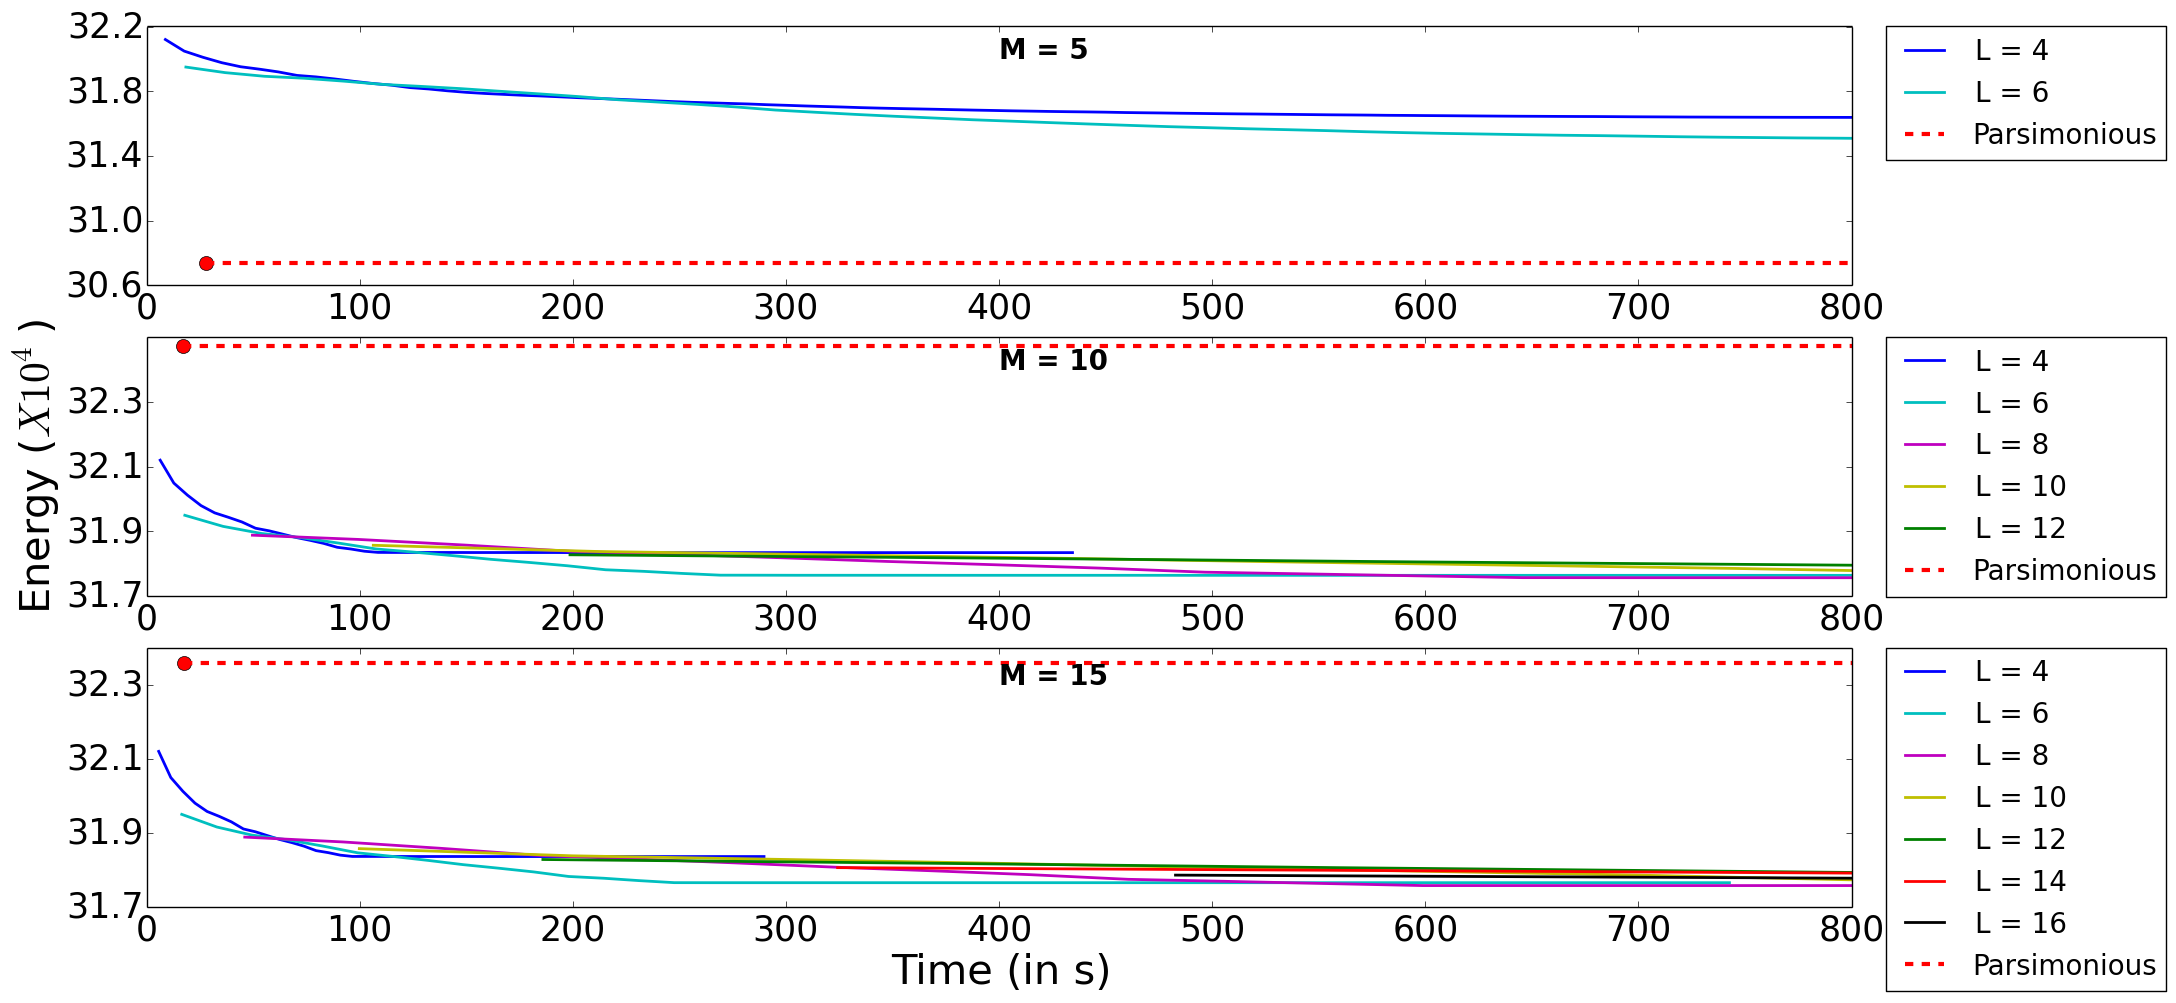
\includegraphics[keepaspectratio = true, width =1.1\textwidth]{\imagePath/synthetic_results/linear_w5}
}
\vspace{3mm}
\mycaption{\footnotesize \em Results for synthetic data using truncated linear distance function. The plots show the variation of energy versus time, averaged over 50 lattices using $\omega_c = 5$. We use truncation factors as $M$ = 5, 10 and 15  and $m$ = 1, and for each we vary interval lengths for our algorithm. This plot is the same as shown in the paper, but we include it here for the sake of comparison. Red dot indicates convergence of parsimonious labeling algorithm and dotted line indicates extrapolation.}
\label{fig:linear_weight5}
\end{figure*}

\begin{figure*}
\centerline{
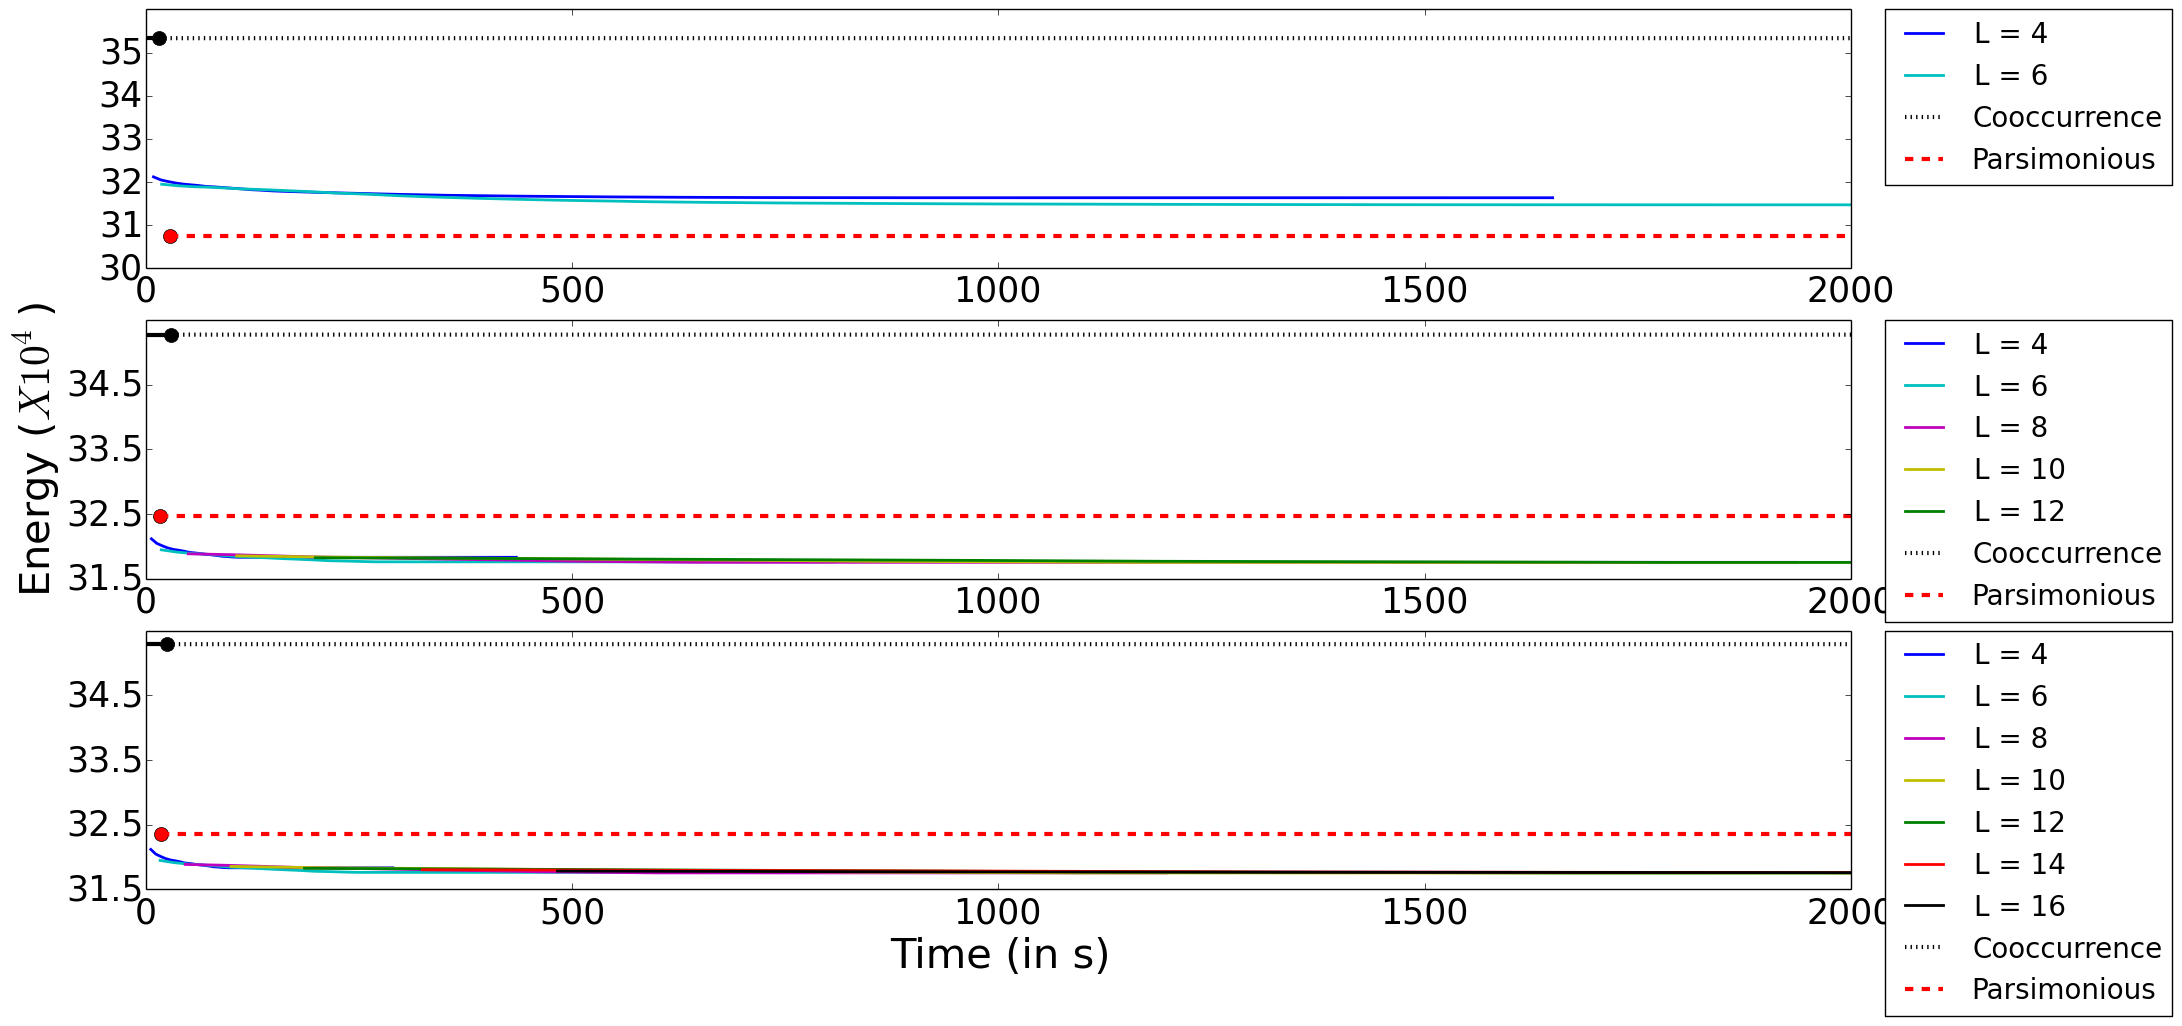
\includegraphics[keepaspectratio = true, width =1.1\textwidth]{\imagePath/synthetic_results/linear_w5_cooc}
}
\vspace{3mm}
\mycaption{\footnotesize \em Results for synthetic data using truncated linear distance function. The plots show the variation of energy versus time, averaged over 50 lattices using $\omega_c = 5$. We use truncation factors as $M$ = 5, 10 and 15  and $m$ = 1, and for each we vary interval lengths for our algorithm. This plot corresponds to the same experiment as mentioned in the paper, but with results for co-occurrence included. Red and black dots indicate convergence of respective algorithms and dotted line indicates extrapolation.}
\label{fig:linear_weight5_cooc}
\end{figure*}

\begin{figure*}
\centerline{
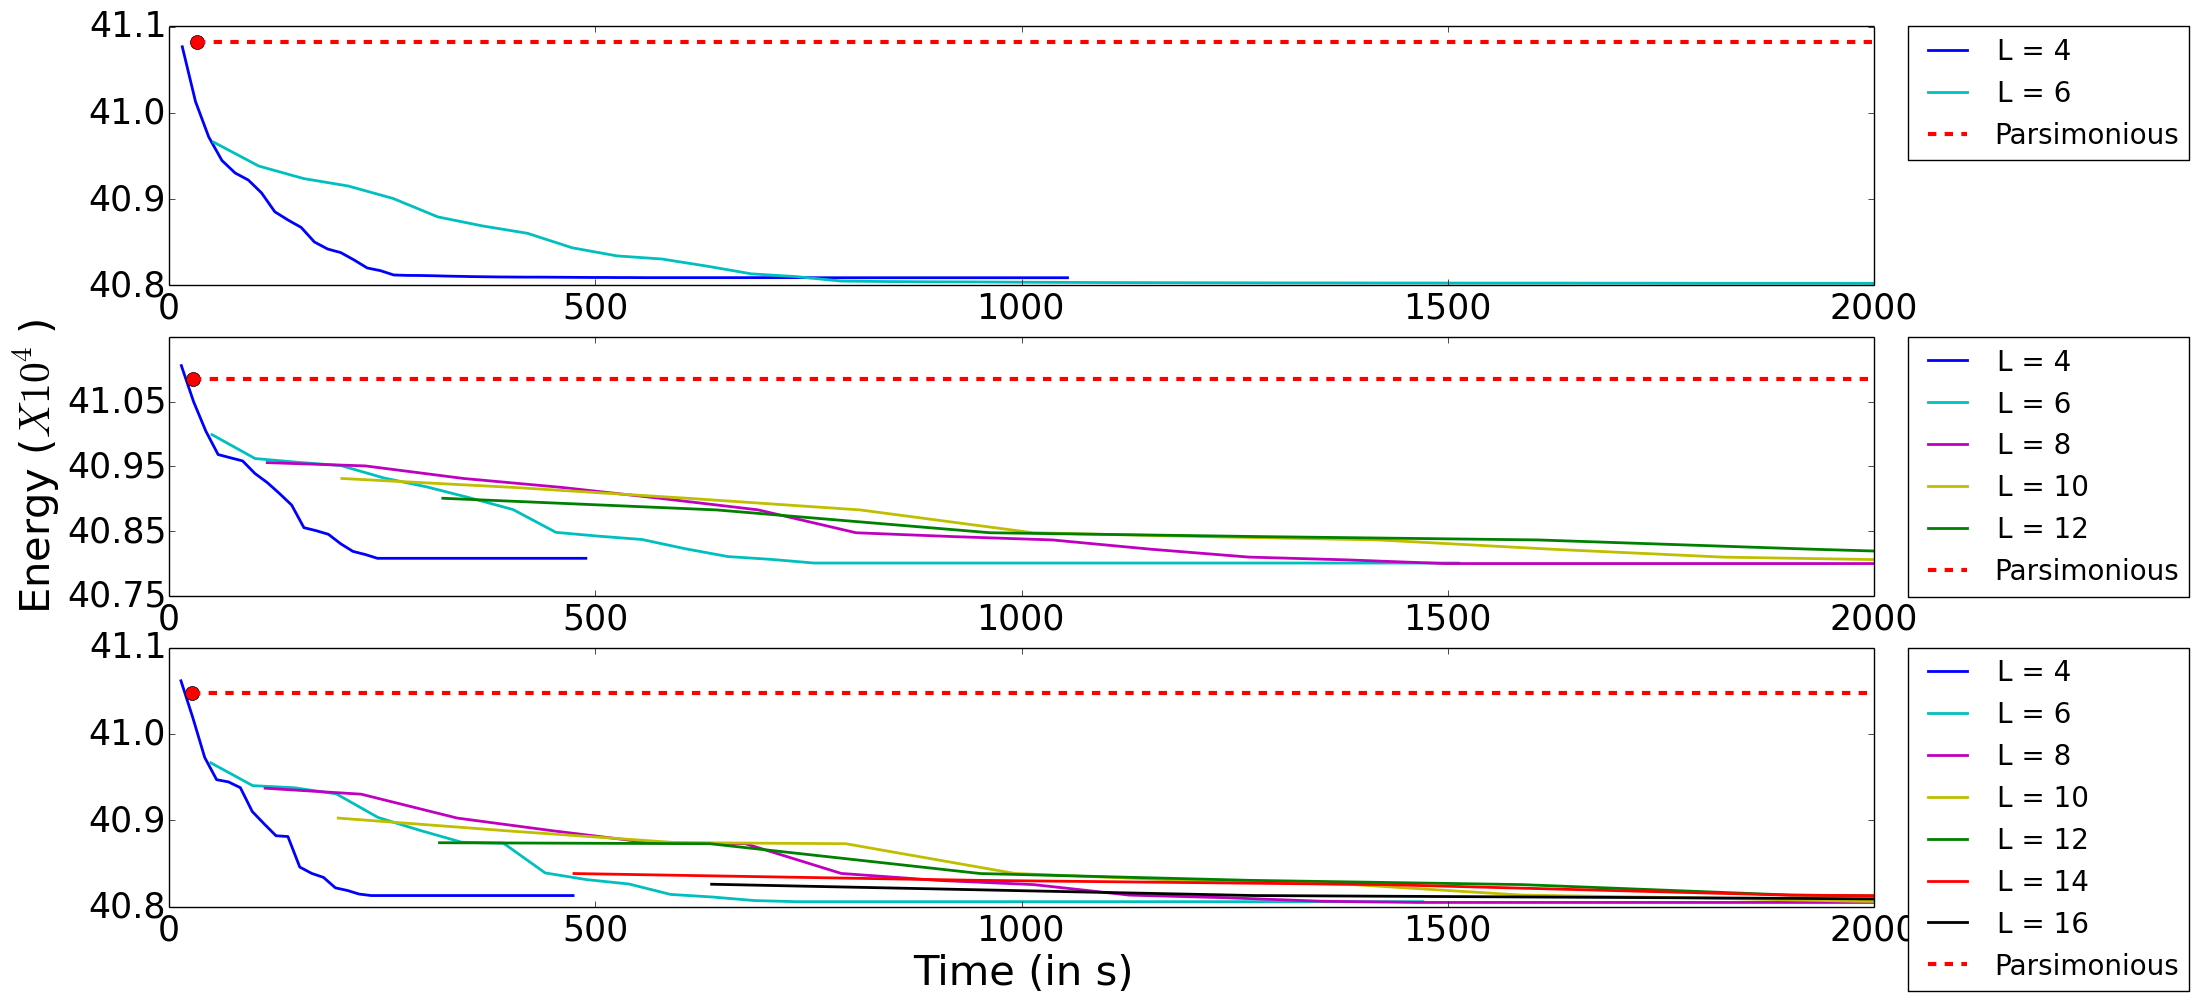
\includegraphics[keepaspectratio = true, width =1.1\textwidth]{\imagePath/synthetic_results/linear_w10}
}
\vspace{3mm}
\mycaption{\footnotesize \em Results for synthetic data using truncated linear distance function. The plots show the variation of energy versus time, averaged over 50 lattices using $\omega_c = 10$. We use truncation factors as $M$ = 5, 10 and 15  and $m$ = 1, and for each we vary interval lengths for our algorithm. Parsimonious labeling performs well for $M$ = 5, but our approach outperforms for higher values of $M$. Red dot indicates convergence of parsimonious labeling and dotted line indicates extrapolation.}
\label{fig:linear_weight10}
\end{figure*}


\begin{figure*}
\centerline{
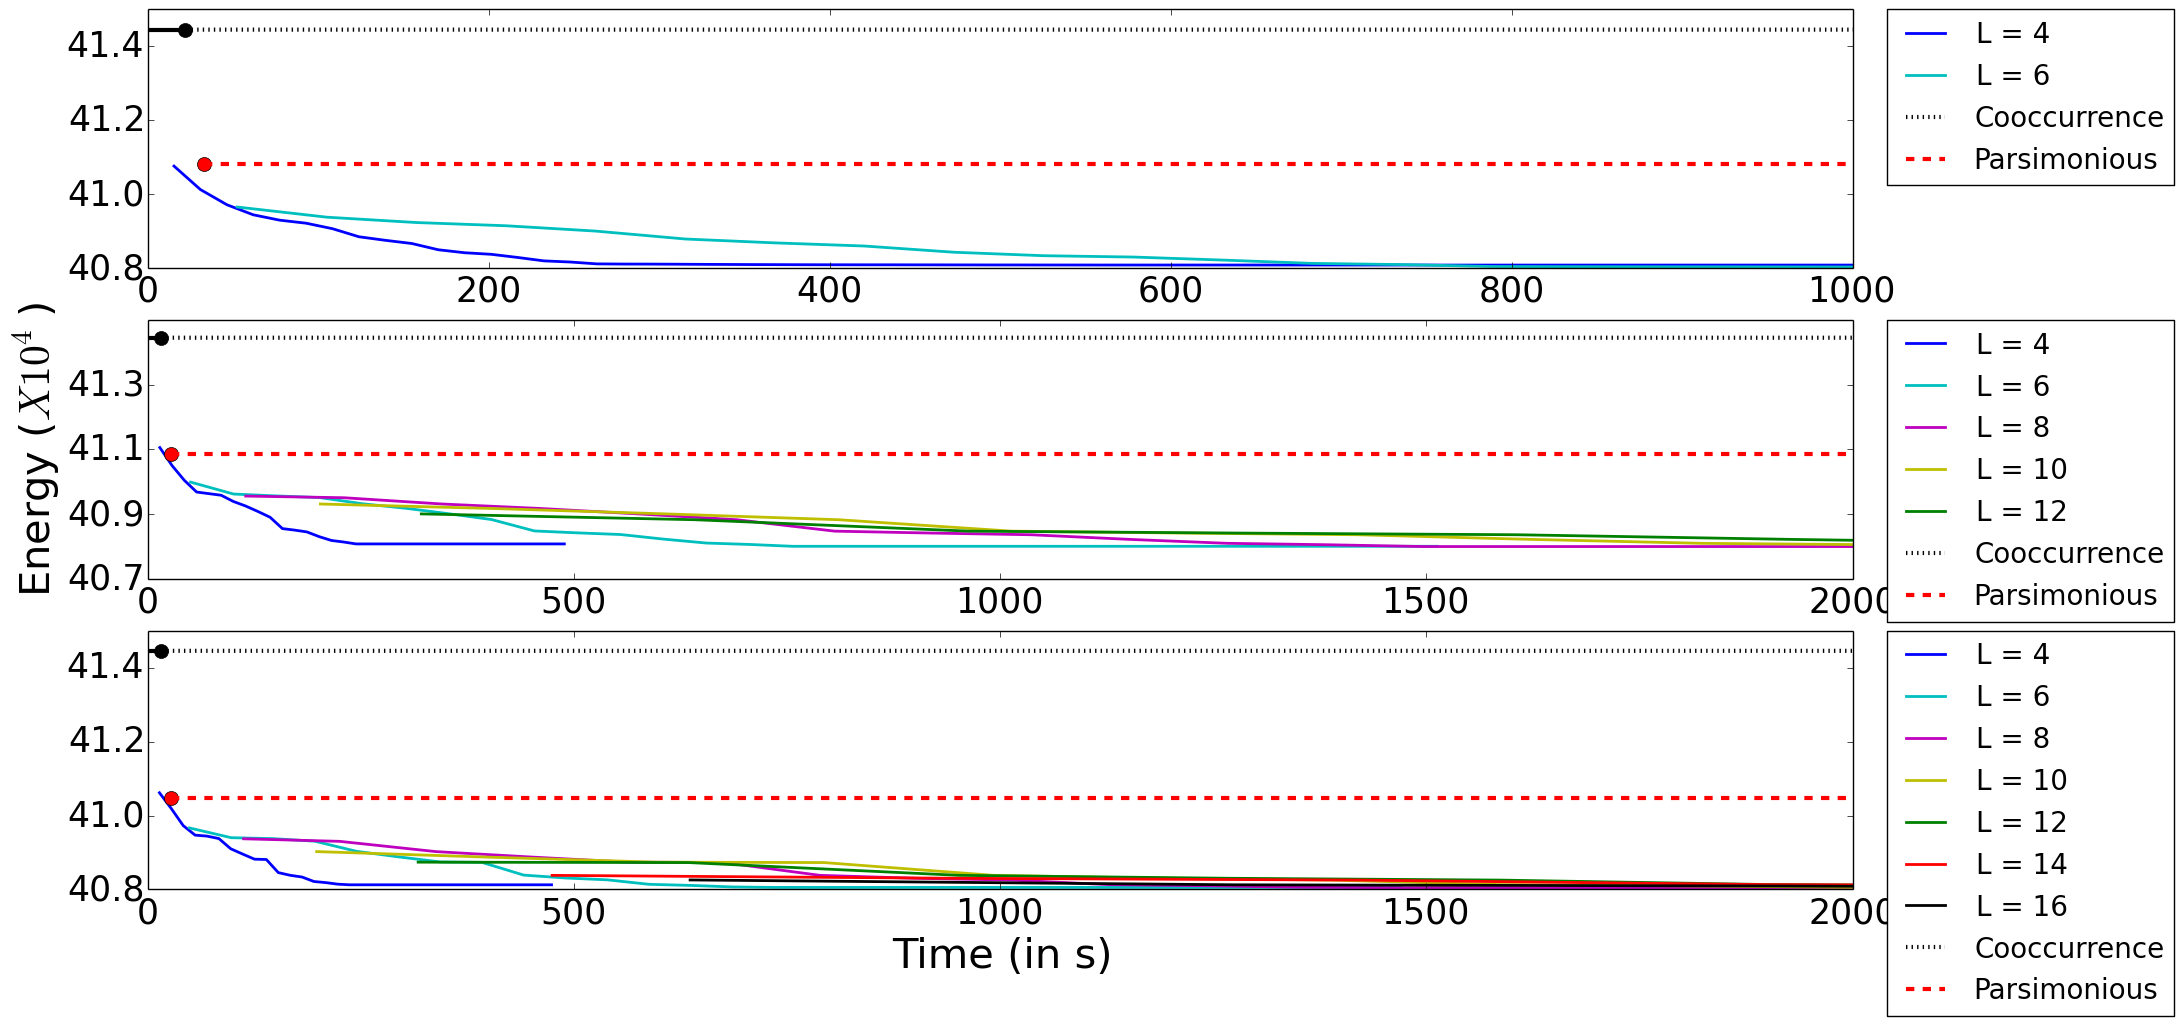
\includegraphics[keepaspectratio = true, width =1.1\textwidth]{\imagePath/synthetic_results/linear_w10_cooc}
}
\vspace{3mm}
\mycaption{\footnotesize \em Results for synthetic data using truncated linear distance function. The plots show the variation of energy versus time, averaged over 50 lattices using $\omega_c = 5$. We use truncation factors as $M$ = 5, 10 and 15  and $m$ = 1, and for each we vary interval lengths for our algorithm. This plot corresponds to the same experiment as in figure ~\ref{fig:linear_weight10}, but with results for co-occurrence included. Red and black dots indicate convergence of respective algorithms and dotted line indicates extrapolation.}
\label{fig:linear_weight10_cooc}
\end{figure*}

\begin{figure*}
\centerline{
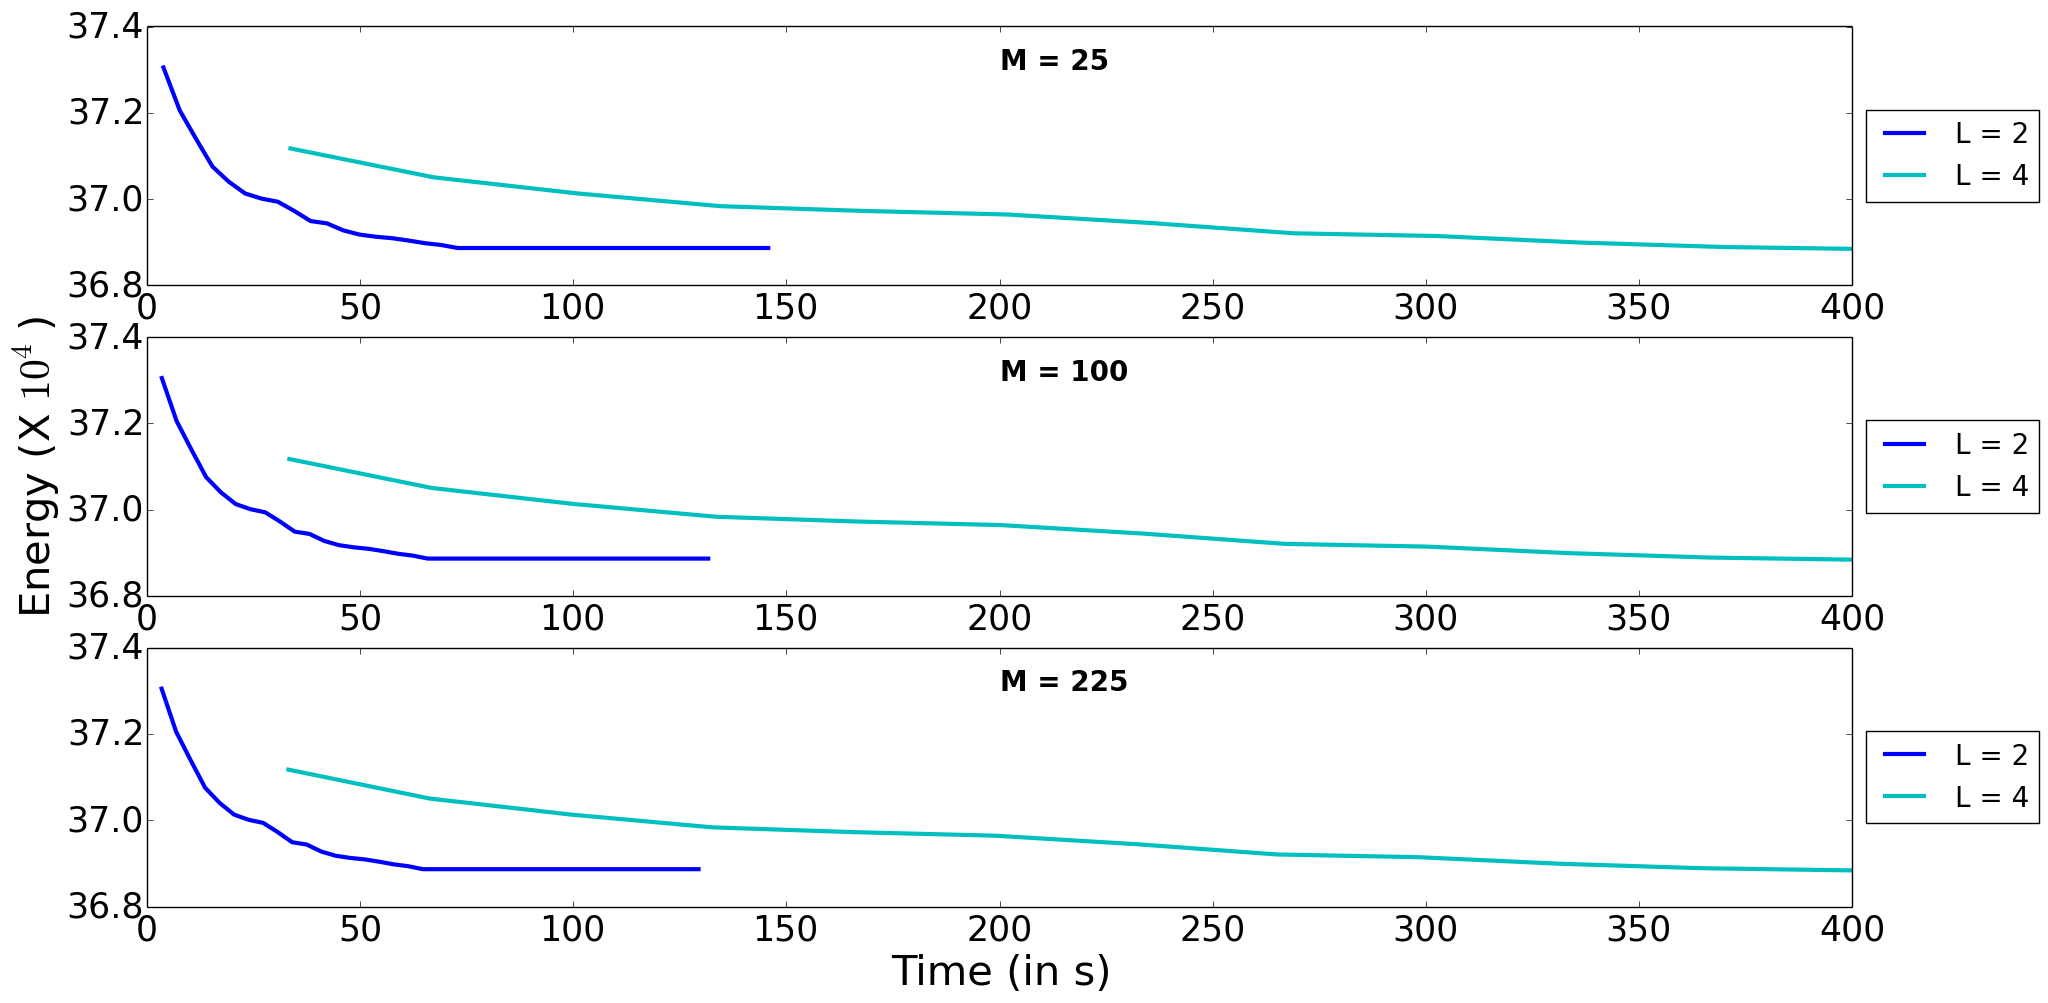
\includegraphics[keepaspectratio = true, width = 1.1\textwidth]{\imagePath/synthetic_results/quadratic_w5}
}
\vspace{3mm}
\mycaption{\footnotesize \em Results for synthetic data using truncated quadratic distance function. The plots show the variation of energy versus time, averaged over 50 lattices using $\omega_c = 5$. We use $M$ = 25, 100 and 225, and for each we vary interval lengths for our algorithm.}
\label{fig:quadratic_weight5}
\end{figure*}

\myparagraph{\bf Data.} We generate lattices of size 100 $\times$ 100, where each lattice point represents a variable taking one of 20 labels. The cliques are defined as all 10 $\times$ 10 subwindows. The unary potentials are uniformly sampled in the range [1, 100]. The truncation factors for linear case are $M \in \{5, 10, 15\}$ and for quadratic case $M \in \{25, 100, 225\}$. In each energy function, all cliques were assumed to have the same clique weight, being 5 and 10 for linear model, and 3 and 5 for quadratic model. We use $m = 1$ for the sake of comparison with ~\cite{dokaniaiccv15} and~\cite{ladickyeccv10}. %Note that we used clique weights as 5 for linear model and 3 for quadratic model in the paper.

\myparagraph{\bf Method.} For each energy function obtained by a particular setting of the above parameters, we vary the interval length up to $M$ + 1. We run~\cite{dokaniaiccv15} and~\cite{ladickyeccv10} only for linear distance function and $m$ = 1. The experiments are repeated for 50 randomly generated unaries for linear and quadratic cases. 

\myparagraph{\bf Results.} The plots in Figure~\ref{fig:linear_weight5_cooc} and ~\ref{fig:linear_weight5} show the average energy as a function of average time for our algorithm and the baselines using weight as 5 for max-of-linear models, with and without the results of ~\cite{ladickyeccv10} respectively. We see that the energy values of  ~\cite{ladickyeccv10} are much higher as compared to our algorithm. Our algorithm gives lower energy solutions than parsimonious labeling method except when the truncation factor is low ($M$ = 5). The plots in Figures~\ref{fig:linear_weight10_cooc} and ~\ref{fig:linear_weight10} shows the results for max-of-linear models using weight as 10 with and without the cooccurrence results respectively. Our algorithm gives better results than the baselines for all $M$. Both the baselines converge faster than our method. In practice, intervals smaller than the optimum size give almost equally good results and converge faster. Figure~\ref{fig:quadratic_weight5} shows the plot for max-of-quadratic cases using weight as 5.

\clearpage
\mysubsection{Real Data}

We present results on the two problems of image inpainting and denoising, and stereo matching. These enable us to visually infer the quality of our solutions. We use the energy of final labeling and convergence time as the evaluation criteria. 

\mysubsubsection{Image Inpainting and Denoising}

%	\scriptsize(f) House input & \scriptsize(g) Cooccurrence & \scriptsize(h) Parsimonious & \scriptsize(i) $m$ = 1, $L$ = 20 & \scriptsize(j) $m$ = 3, $L$ = 20\\
%	\scriptsize(Energy, Time (s)) & \scriptsize(42018464, 486) & \scriptsize(37349032, 12024) & \scriptsize(36903599, 22751) & \scriptsize($37093699^*$, 23260)\\

\myparagraph{\bf Data.} Given an image with noise and obscured/inpainted regions (regions with missing pixels), the task is to denoise it and fill the obscured regions in a way that is consistent with the surrounding regions. The images `house' and `penguin' from the Middlebury data set were used for the experiments. Since the images are grayscale, they have 256 labels in the interval [0, 255], each representing an intensity value. The unary potential for each pixel corresponding to a particular label equals the squared difference between the label and the intensity value at the pixel. We use high-order cliques as the super-pixels obtained using the mean-shift method~\cite{comaniciu2002mean}. The parameters $\omega_c$, $M$ and $m$ are varied to give different truncated max-of-linear energy functions.

\myparagraph{\bf Method.} For each parameter setting of $\omega_c$, $M$ and $m$, we vary the interval lengths for our algorithm and make a comparison with the baselines.

\myparagraph{\bf Results.} Results for $\omega_c$ = 40, $M$ = 40, and $m$ = 1, 3 and 5 for `penguin' and $\omega_c$ = 50, $M$ = 50, and $m$ = 1, 3 and 5 for `house' are shown in Figure~\ref{fig:inpainting_results} for varying interval lengths $L = \{5, 10, 20\}$. Note that we showed results for only $L = 20$ in the main paper. Our algorithm consistently gives lower energy labeling as compared to both~\cite{dokaniaiccv15} and~\cite{ladickyeccv10} even for small $L$. For `penguin', our algorithm gives cleaner denoised image, preserving edges and details. On the other hand, both~\cite{dokaniaiccv15} and~\cite{ladickyeccv10} exhibit significant blocking effect. Moreover, the output is more natural for $m$ = 3 as compared to $m$ = 1. Even for `house', our output looks more visually appealing as compared to baselines.

\begin{figure}[t]
	\centering
\begin{tabular}{ccc}
	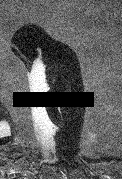
\includegraphics[scale = 0.60]{\imagePath/inpainting_results/penguin-input} &
	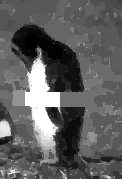
\includegraphics[scale = 0.60]{\imagePath/inpainting_results/penguin_COOC_w40_M40} &
	
\includegraphics[scale = 0.60]{\imagePath/inpainting_results/penguin_HIER_w40_M40}\\
	\scriptsize{(a) Penguin input} & \scriptsize{(b) Cooccurrence} & \scriptsize{(c) Parsimonious} \\ 
	\scriptsize(Energy, Time (s)) & \scriptsize(14735411, 237) & \scriptsize(12585846, 456) \\ 
	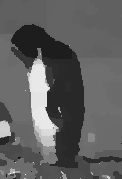
\includegraphics[scale = 0.60]{\imagePath/inpainting_results/confFileInpainting_penguinL5_m1_M40_wc40_labeling} &
	
\includegraphics[scale = 0.60]{\imagePath/inpainting_results/confFileInpainting_penguinL10_m1_M40_wc40_labeling} &
	
\includegraphics[scale = 0.60]{\imagePath/inpainting_results/confFileInpainting_penguinL20_m1_M40_wc40_labeling} \\ 
	\scriptsize{(d) $m$ = 1, $L$ = 5} & \scriptsize{(e) $m$ = 1, $L$ = 10} & \scriptsize{(f) $m$ = 1, $L$ = 20} \\ 
	\scriptsize(12541999, 1694) & \scriptsize(123598999, 2633) & \scriptsize(123018999, 3963) \\
	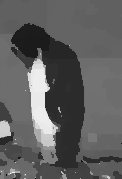
\includegraphics[scale = 0.60]{\imagePath/inpainting_results/confFileInpainting_penguinL5_m3_M40_wc40_labeling} &
	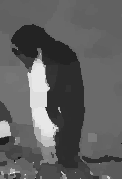
\includegraphics[scale = 0.60]{\imagePath/inpainting_results/confFileInpainting_penguinL10_m3_M40_wc40_labeling} &
	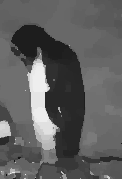
\includegraphics[scale = 0.60]{\imagePath/inpainting_results/confFileInpainting_penguinL20_m3_M40_wc40_labeling} \\ 
	\scriptsize{(g) $m$ = 3, $L$ = 5} & \scriptsize{(h) $m$ = 3, $L$ = 10} & \scriptsize{(i) $m$ = 3, $L$ = 20} \\ 
	\scriptsize(126481999, 1379) & \scriptsize(125784999, 2499) & \scriptsize(124044999, 5018) \\
	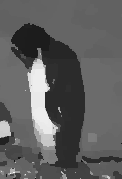
\includegraphics[scale = 0.60]{\imagePath/inpainting_results/confFileInpainting_penguinL5_m5_M40_wc40_labeling} &
	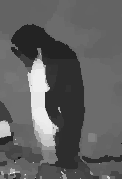
\includegraphics[scale = 0.60]{\imagePath/inpainting_results/confFileInpainting_penguinL10_m5_M40_wc40_labeling} &
	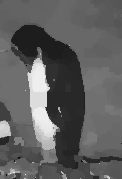
\includegraphics[scale = 0.60]{\imagePath/inpainting_results/confFileInpainting_penguinL20_m5_M40_wc40_labeling} \\ 
	\scriptsize{(j) $m$ = 5, $L$ = 5} & \scriptsize{(k) $m$ = 5, $L$ = 10} & \scriptsize{(l) $m$ = 5, $L$ = 20} \\ 
	\scriptsize(127329999, 1357) & \scriptsize(125284999, 2367) & \scriptsize(124501999, 5706) \\
\end{tabular}
\mycaption{\footnotesize \em Image inpainting results for `penguin'. Note that comparison with (b) and (c) makes sense only for $m$ = 1. Also, we restricted our experiments to smaller (and suboptimal) $L$ due to computational issues.}
\label{fig:inpainting_results}
\end{figure}

\begin{figure}[t]
	\centering
\begin{tabular}{ccc}
	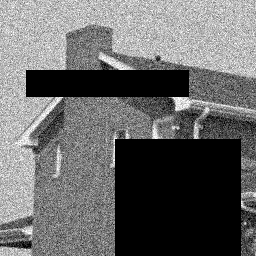
\includegraphics[scale = 0.40]{\imagePath/inpainting_results/house-input} &
	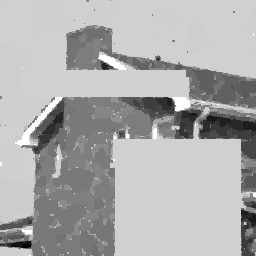
\includegraphics[scale = 0.40]{\imagePath/inpainting_results/house_COOC_w50_M50} &
	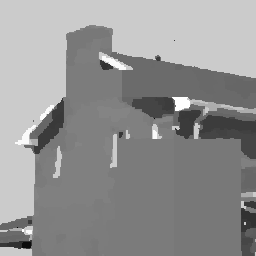
\includegraphics[scale = 0.40]{\imagePath/inpainting_results/house_HIER_w50_M50}\\
	\scriptsize{(a) Penguin input} & \scriptsize{(b) Cooccurrence} & \scriptsize{(c) Parsimonious} \\ 
	\scriptsize(Energy, Time (s)) & \scriptsize(42018464, 486) & \scriptsize(37349032, 12024) \\ 
	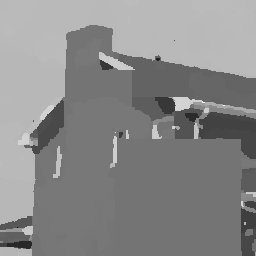
\includegraphics[scale = 0.40]{\imagePath/inpainting_results/confFileInpainting_houseL5_m1_M50_wc50_labeling} &
	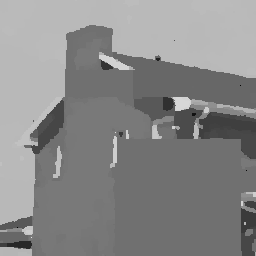
\includegraphics[scale = 0.40]{\imagePath/inpainting_results/confFileInpainting_houseL10_m1_M50_wc50_labeling} &
	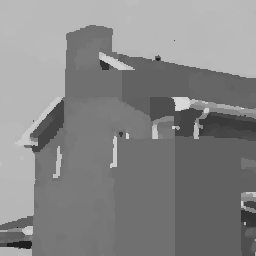
\includegraphics[scale = 0.40]{\imagePath/inpainting_results/confFileInpainting_houseL20_m1_M50_wc50_labeling} \\ 
	\scriptsize{(d) $m$ = 1, $L$ = 5} & \scriptsize{(e) $m$ = 1, $L$ = 10} & \scriptsize{(f) $m$ = 1, $L$ = 20} \\ 
	\scriptsize(37196999, 8084) & \scriptsize(370873999, 11356) & \scriptsize(369035999, 22752) \\
	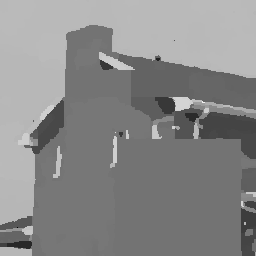
\includegraphics[scale = 0.40]{\imagePath/inpainting_results/confFileInpainting_houseL5_m3_M50_wc50_labeling} &
	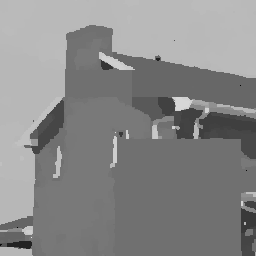
\includegraphics[scale = 0.40]{\imagePath/inpainting_results/confFileInpainting_houseL10_m3_M50_wc50_labeling} &
	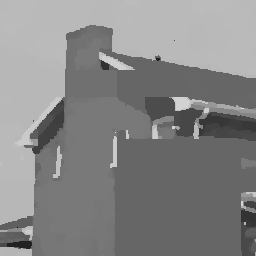
\includegraphics[scale = 0.40]{\imagePath/inpainting_results/confFileInpainting_houseL20_m3_M50_wc50_labeling} \\ 
	\scriptsize{(g) $m$ = 3, $L$ = 5} & \scriptsize{(h) $m$ = 3, $L$ = 10} & \scriptsize{(i) $m$ = 3, $L$ = 20} \\ 
	\scriptsize(373067999, 7744) & \scriptsize(37115999, 9547) & \scriptsize(370936999, 23261) \\
	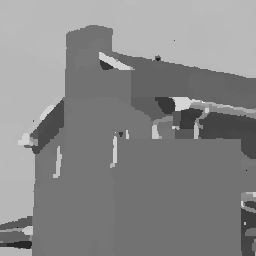
\includegraphics[scale = 0.40]{\imagePath/inpainting_results/confFileInpainting_houseL5_m5_M50_wc50_labeling} &
	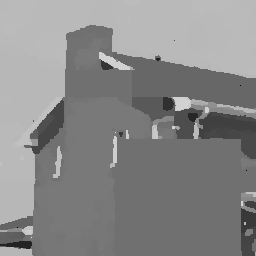
\includegraphics[scale = 0.40]{\imagePath/inpainting_results/confFileInpainting_houseL10_m5_M50_wc50_labeling} &
	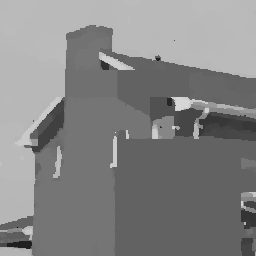
\includegraphics[scale = 0.40]{\imagePath/inpainting_results/confFileInpainting_houseL20_m5_M50_wc50_labeling} \\ 
	\scriptsize{(j) $m$ = 5, $L$ = 5} & \scriptsize{(k) $m$ = 5, $L$ = 10} & \scriptsize{(l) $m$ = 5, $L$ = 20} \\ 
	\scriptsize(374691999, 6476) & \scriptsize(372811999, 9949) & \scriptsize(375026999, 22985) \\
\end{tabular}
\vspace{2mm}
\mycaption{\footnotesize \em Image inpainting results for `house'. Note that comparison with (b) and (c) makes sense only for $m$ = 1. Also, we restricted our experiments to smaller (and suboptimal) $L$ due to computational issues.}
\label{fig:inpainting_results}
\end{figure}

\clearpage

\mysubsubsection{Stereo Matching}

\myparagraph{\bf Data.} In the stereo matching problem, we have two rectified images of the same scene from two cameras set slightly apart. We are required to estimate the horizontal disparity between a pixel in the right camera image from the corresponding pixel in the left camera. We use `tsukuba', `teddy', `venus' and `cones' datasets from the Middlebury stereo collection for our experiments. In each case, we have a pair of RGB images and ground truth disparities. We assume the unary potentials to be the $L1$-norm of the difference in RGB values of the left and right image pixels. There are 16 labels and 60 labels for `tsukuba' and `teddy' respectively. The high-order cliques are super-pixels obtained using mean-shift method~\cite{comaniciu2002mean}. The parameters $\omega_c$, $M$ and $m$ are varied to give different truncated max-of-linear energy functions.


\myparagraph{\bf Method.} For each parameter setting of $\omega_c$, $M$ and $m$, we vary the interval lengths for our algorithm and make a comparison with the baselines.

\myparagraph{\bf Results.} Results for $\omega_c$ = 20, $M$ = 5, and $m$ = 1 and 3 for `tsukuba', `venus' and `cones', and $\omega_c$ = 20, $M$ = 1, and $m$ = 1 and 3 for `teddy' are shown in Figure~\ref{fig:stereo_matching}. We show the results for interval length 3 for `teddy', and 6 for others. Note that in our main paper, we used interval length $L$ as 4 for `tsukuba' and `venus', and 1 for `teddy' and did not show the results for `cones'. Apart from `cones', our algorithm consistently gives lower energy labeling as compared to both~\cite{dokaniaiccv15} and~\cite{ladickyeccv10}. 

\clearpage
\newgeometry{left=4cm,right=4cm,bottom=3cm,right=3cm}

\begin{figure}[t]
	\centering
\begin{tabular}{ccccc}
	
\includegraphics[scale = 0.17]{\imagePath/stereo_results/tsukuba_groundtruth} &
	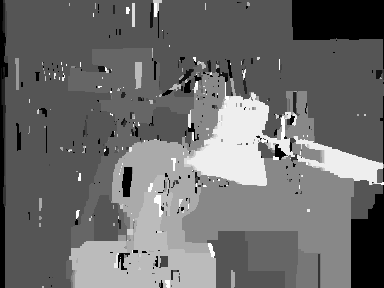
\includegraphics[scale = 0.17]{\imagePath/stereo_results/tsukuba_COOC_M5_wc20} &
	
\includegraphics[scale = 0.17]{\imagePath/stereo_results/tsukuba_HIER_M5_wc20} &
	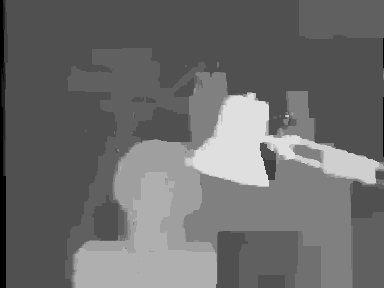
\includegraphics[scale = 0.17]{\imagePath/stereo_results/confFileStereo_tsukubaL6_m1_M5_wc20_labeling} &
	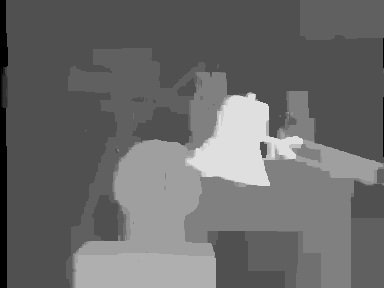
\includegraphics[scale = 0.17]{\imagePath/stereo_results/confFileStereo_tsukubaL6_m3_M5_wc40_labeling} \\
	\scriptsize(a) Ground truth & \scriptsize(b) Cooccurrence & \scriptsize(c) Parsimonious & \scriptsize(d) $m$ = 1, $L$ = 6 & \scriptsize(e) $m$ = 3, $L$ = 6 \\
	\scriptsize(Energy, Time (s)) & \scriptsize(2098800, 101) & \scriptsize(1364200, 225) & \scriptsize(1258499, 518) & \scriptsize(1391629, 720) \\ 
	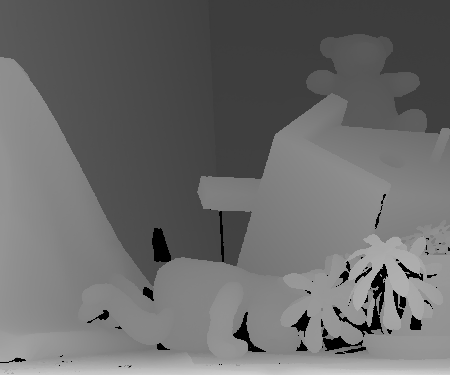
\includegraphics[scale = 0.15]{\imagePath/stereo_results/teddy_groundtruth} &
	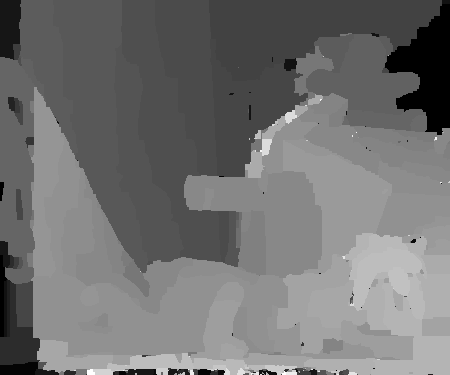
\includegraphics[scale = 0.15]{\imagePath/stereo_results/teddy_COOC_M1_wc20} &
	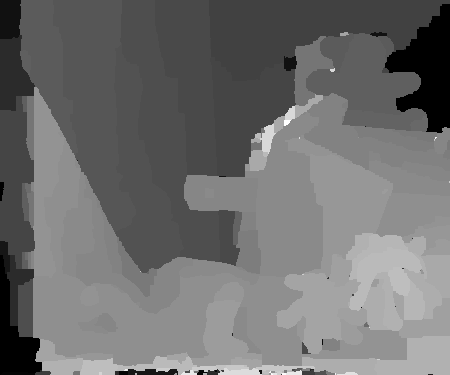
\includegraphics[scale = 0.15]{\imagePath/stereo_results/teddy_HIER_M1_wc20} &
	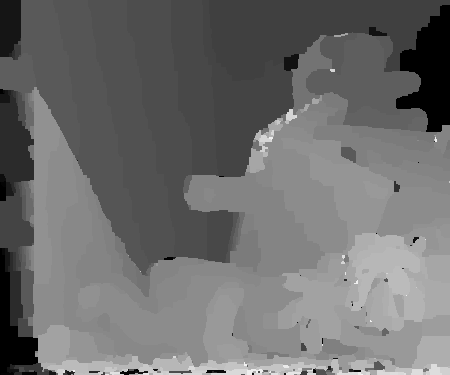
\includegraphics[scale = 0.15]{\imagePath/stereo_results/confFileStereo_teddyL3_m1_M1_wc20_labeling} &
	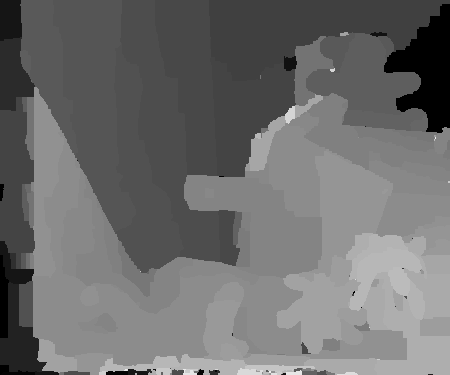
\includegraphics[scale = 0.15]{\imagePath/stereo_results/confFileStereo_teddyL3_m3_M1_wc20_labeling} \\
	\scriptsize(f) Ground truth & \scriptsize(g) Cooccurrence & \scriptsize(h) Parsimonious & \scriptsize(i) $m$ = 1, $L$ = 3 & \scriptsize(j) $m$ = 3, $L$ = 3 \\
	\scriptsize(Energy, Time (s)) & \scriptsize(3259900, 495) & \scriptsize(3201300, 484) & \scriptsize(3202489, 6216) & \scriptsize(3211819, 5043) \\ 
	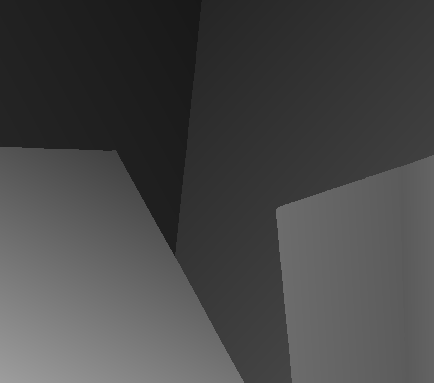
\includegraphics[scale = 0.15]{\imagePath/stereo_results/venus_groundtruth} &
	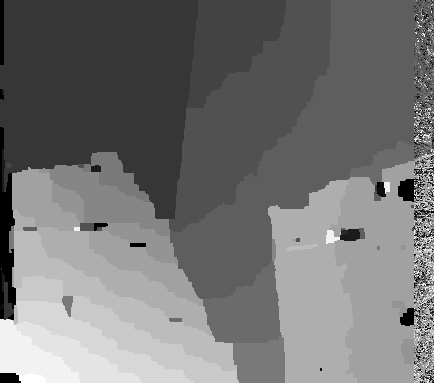
\includegraphics[scale = 0.15]{\imagePath/stereo_results/venus_COOC_M5_wc20} &
	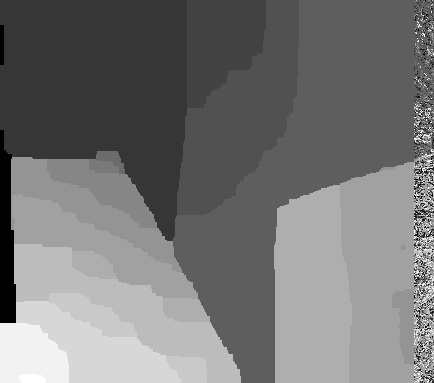
\includegraphics[scale = 0.15]{\imagePath/stereo_results/venus_HIER_M5_wc20} &
	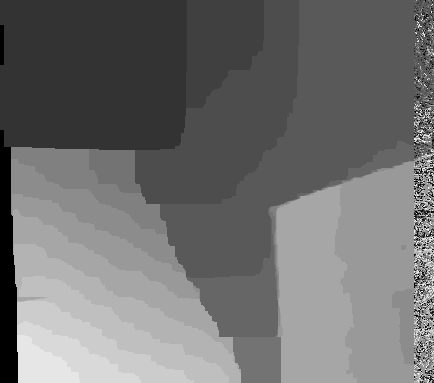
\includegraphics[scale = 0.15]{\imagePath/stereo_results/confFileStereo_venusL6_m1_M5_wc20_labeling} &
	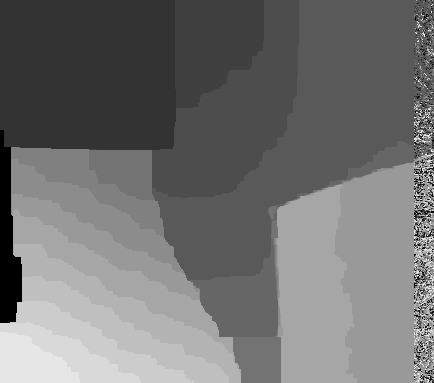
\includegraphics[scale = 0.15]{\imagePath/stereo_results/confFileStereo_venusL6_m3_M5_wc20_labeling} \\
	\scriptsize(k) Ground truth & \scriptsize(l) Cooccurrence & \scriptsize(m) Parsimonious & \scriptsize(n) $m$ = 1, $L$ = 6 & \scriptsize(o) $m$ = 3, $L$ = 6 \\
	\scriptsize(Energy, Time (s)) & \scriptsize(2343200, 261) & \scriptsize(2262600, 482) & \scriptsize(2207549, 4624) & \scriptsize(2222299, 4189) \\ 
	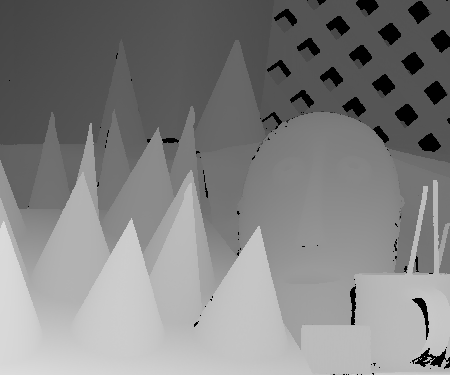
\includegraphics[scale = 0.15]{\imagePath/stereo_results/cone_groundtruth} &
	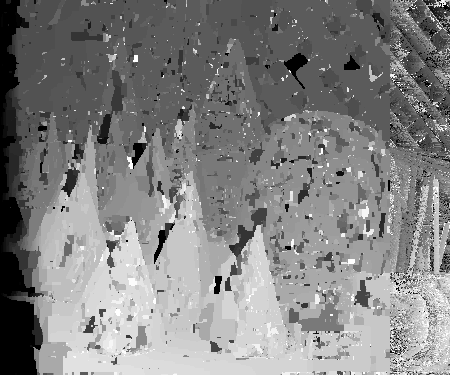
\includegraphics[scale = 0.15]{\imagePath/stereo_results/cone_COOC_M5_wc20} &
	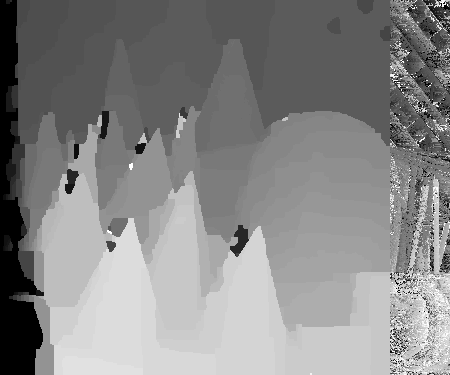
\includegraphics[scale = 0.15]{\imagePath/stereo_results/cone_HIER_M5_wc20} &
	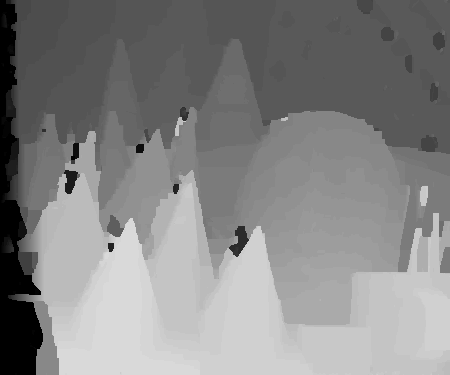
\includegraphics[scale = 0.15]{\imagePath/stereo_results/confFileStereo_coneL6_m1_M5_wc20_labeling} &
	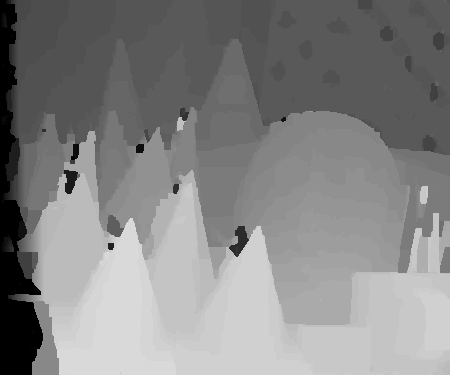
\includegraphics[scale = 0.15]{\imagePath/stereo_results/confFileStereo_coneL6_m3_M5_wc20_labeling} \\
	\scriptsize(p) Ground truth & \scriptsize(q) Cooccurrence & \scriptsize(r) Parsimonious & \scriptsize(s) $m$ = 1, $L$ = 6 & \scriptsize(t) $m$ = 3, $L$ = 6 \\
	\scriptsize(Energy, Time (s)) & \scriptsize(8260100, 308) & \scriptsize(4985639, 759) & \scriptsize(5237919, 3711) & \scriptsize(5258999, 4137) \\ 

\end{tabular}
\mycaption{\footnotesize \em Stereo matching results: Figures (a), (f), (k) and (p) are the ground truth disparity for `tsukuba', `teddy', `venus' and `cones' respectively. Our results for $m$ = 1 (d), (i), (n) and (s) are significantly better than those of~\cite{ladickyeccv10} (b), (g), (l) and (q), and of~\cite{dokaniaiccv15} (c), (h), (m) and (r) in terms of energy. We also show results for $m$ = 3. We use super-pixels obtained using mean-shift as cliques. $^*$Note that $m$ = 3 uses a different energy function from other cases.}
\label{fig:stereo_matching}
\end{figure}

\clearpage
\restoregeometry

\section{Advantages of using TMCM}

\begin{table}[h!]
\begin{center}

\begin{tabular}{|r|c|c|c|}
\hline
Labeling & $m=1$ & $m=2$ & $m=3$ \\
\hline
(a) \{1,1,1,1,2,2\} & 1 & 2 & 2 \\
\{1,2,3,4,5,6\} & 3 & 6 & 7 \\
\hline
(b) \{1,1,1,9,9,9\} & 3 & 6 & 9 \\
\{1,1,1,8,8,9\} & 3 & 6 & 9 \\
\hline
(c) \{1,1,1,1,1,7\} & 3 & 3 & 3 \\
\{1,1,1,2,3,4\} & 3 & 5 & 6 \\
\hline
\end{tabular}

\mycaption{\footnotesize \em Clique potential value $\theta_{\bf c}({\bf x}_{\bf c})$ defined by a linear function with $M$ = 3 and $\bf{\omega_c}$ = 1 for various
		values of $m$. Since clique size is 6, $0 \leq m \leq 3$. Pair (a)
		demonstrates why taking the largest convex distances favors smoothness; (b) demonstrates how truncation prevents overpenalization of
		discontinuities; (c) demonstrates how using $m > 1$ can provide some degree of robustness to errors in the definitions of the cliques.
}
\label{table:cliqueExample}
\end{center}
\end{table}

\myparagraph{\bf Smoothness.} The truncated max-of-convex potentials encourage smooth labelings. In order to illustrate this, let us consider the
example of a clique of six random variables ${\bf X}_{\bf c}$ and a label set ${\bf L}$ of size $10$. We can define a truncated convex distance
using a linear function $d(y) = |y|$ and a truncation factor of $M=3$. Consider pair (a) of labelings shown
in table~\ref{table:cliqueExample}. If the labeling is \{1, 1, 1, 1, 2, 2\} and $M$ = 3, $m$ = 3, $\bf\omega_c$ = 1, $\theta_{\bf c}({\bf x}_{\bf c})$ = min(6-1, 3) + min(5 - 2, 6) + min(4 - 3, 3) = 3 + 3 + 1 = 7. Clearly, the first labeling of this pair is significantly smoother than the second, which is reflected in the value of the
clique potential for all values of $m$. In contrast, if we were to consider the minimum distance among all pairs of labels, both the labelings will
provide a clique potential value of $0$.  
\vspace{-1mm}

\myparagraph{\bf Discontinuities.} Similar to the pairwise case, the use of a truncation factor helps prevent overpenalization of discontinuities. For example,
let us consider the pair (b) of labelings in table~\ref{table:cliqueExample}. In both cases, the six random variables appear to belong to two
{\em groups}, one whose labels are low and one whose labels are high. Without a truncation, such a discontinuity would have been penalized heavily (for example,
8 for $m=1$ for both the labelings). This in turn would discourage the clique to be assigned this labeling even though this type of discontinuity is expected
to occur in natural images. However, with a truncation, the penalty is significantly less (for example, 3 for $m=1$ for both the labelings), which can help
preserve the discontinuities in the labeling obtained via energy minimization.
\vspace{-1mm}

\myparagraph{\bf Robustness.} In order to use a TMCM, we would be required to define the cliques. For example, given an image, we could use a bottom-up oversegmentation
approach to obtain superpixels, and then set all the pixels in a superpixel to belong to a clique. However, oversegmentation can introduce errors since it has
no notion of the specific vision application we are interested in modeling. To add robustness to errors in the clique definitions, we can set $m > 1$.
For example, consider pair (c) of labelings in table~\ref{table:cliqueExample}. The first of these labelings contains a single
random variable with a very high label, which could be due to the fact that the corresponding pixel has been incorrectly grouped in this superpixel. 
As can be seen from the values of the potential, the
presence of such an erroneous pixel in the superpixel is not heavily penalized when we use $m > 1$. For example, when $m=3$ the value of the clique potential for
the first labeling (with an erroneous pixel) is the same as the second labeling (which is a fairly smooth labeling).

\begin{table}
\begin{center}
\setlength{\tabcolsep}{10pt}
\renewcommand{\arraystretch}{1.3}
\begin{tabular}{|c|l|}
\hline
$n$ & Number of random variables \\ 
$h$ & Number of labels \\ 
$\mathcal{V}$ & $\{1, 2, \dots, \mathit{n}\}$ \\
$\mathbf{L}$ &  $\{1, 2, \dots, \mathit{h}\}$ \\ 
$\mathbf{X}$ & Set of random variables $\{\mathit{X}_a, a \in \mathcal{V}\}$ \\ 
$\mathbf{X_c}$ & Set of random variable belonging to a clique $\{X_a, a \in \mathbf{c} \subseteq \mathcal{V}\}$ \\ 
$\mathbf{x_c}$ & Labeling of clique $\mathbf{c}$ \\ 
$\mathbf{p(x_c)}$ & Sorted list of the labels present in $\mathbf{x_c}$ \\ 
$\mathit{I_n}$ & Interval of consecutive labels $[i_n + 1, j_n]$ \\ 
$\mathit{L}$ & Length of interval, that is, $\mathit{L} = j_n - i_n$ \\ 
$\Gamma_r$ & Set of intervals $\{[0, r], [r + 1, r + \mathit{L}],\dots, [., h - 1]\}$ \\ 
$\mathit{f}$ & Labeling of the random field ($v_a$ takes the label $l_{f(a)}$) \\
$\mathit{f^*}$ & An optimal (MAP) labeling of the random field \\
$\mathit{\theta}_a(i)$ & Unary potential of assigning label $l_i$ to $v_a$ \\
$\mathbf{\omega_c}$ & Weight for clique $\mathbf{X_c}$ \\ 
$\mathit{c}$ & Size of clique $\mathbf{X_c}$ \\ 
$\mathit{d(.)}$ & Convex function used to define distance between two labels \\
$\mathit{M}$ & Truncation factor \\
$\mathit{\theta}_\mathbf{c}(\mathbf{x_c})$ & Clique potential of assigning label $l_i$ to $v_a$ \\
$\mathit{E(f)}$ & Energy of the labeling $f$ \\
$\mathcal{A}\mathit(f, I_n)$ & \{$\mathbf{X_c} \in \mathcal{C} , f(v) \in I_n \forall v \in \mathbf{X_c}$\} \\
$\mathcal{B}\mathit(f, I_n)$ & \{$\mathbf{X_c} \in \mathcal{C} , \exists X_v, X_w \in \mathbf{X_c} | f(v) \in I_n \land f(w) \notin I_n$ \} \\
\hline
\end{tabular}
\end{center}
\caption{Definitions of various symbols used in the supplementary document}
\end{table}


\section{Optimization via Range Expansion}
As max of truncated convex models are a generalization of truncated convex models, it follows that the corresponding energy
minimization problem is NP-hard. If the range expansion algorithm is extended to TMCM, it results in an NP-hard subproblem (specifically problem~\ref{eq:rangeMove} in algorithm~\ref{algo:rangeExpansion}). To overcome this problem, we first overstimate the energy function ${E}$ by a submodular function ${E'}$ which is described in the following subsections. Then we construct a graph which represents ${E'}$ up to an additive constant. This enables us to extend the range expansion algorithm to our more general class
of energy functions.

\subsection{Range Expansion Algorithm for TMCM}

\begin{algorithm}
\small
\caption{The range expansion algorithm for TMCM.}
\begin{algorithmic}[1]
\INPUT Energy function $E(\cdot)$, initial labeling ${\bf x}^0$, interval length $L$.
\STATE Initialize the output labeling $\hat{\bf x} = {\bf x}^0$.
\REPEAT
\FORALL{$i_m \in [-L+2,h]$}
\STATE Define an interval of labels ${\bf I} = \{f,\cdots,l\}$ where $f = \max\{i_m,1\}$ and
$l = \min\{i_m+L-1,h\}$.
\STATE Obtain a new labeling ${\bf x}'$ by solving the following optimization problem:
\begin{eqnarray}
{\bf x}' = && \argmin_{\bf x} E({\bf x}), \nonumber \\
&& \mbox{s.t. } x_a \in {\bf I} \cup \{\hat{x}_a\}, \forall a \in {\cal V}.
\label{eq:rangeMove}
\end{eqnarray}
\IF{$E(\hat{\bf x}) > E({\bf x}')$}
\STATE Update $\hat{\bf x} = {\bf x}'$.
\ENDIF
\ENDFOR
\UNTIL The labeling does not change for any value of $i_m$.
\OUTPUT The labeling $\hat{\bf x}$.
\end{algorithmic}
\label{algo:rangeExpansion}
\end{algorithm}


Algorithm~\ref{algo:rangeExpansion} shows the main steps of the range expansion algorithm. The algorithm starts by assigning
the random variables to an initial label (step 1). For example, all the random variables could be assigned to the label $1$. 
Next, it selects an interval of consecutive labels of size at most $L$ (steps 3-4) where $L$ is specified as an input to the
algorithm. We will see later in the section that the value of $L$ can be chosen to obtain the optimal worst case bound for specific instances of
the max of truncated convex models. Next, it obtains a new labeling that minimizes the energy over all the labelings that either allow a random
variable to retain its current label, or choose a new label in the selected interval (step 5). If the energy of the new labeling is lower than
that of the current labeling, then the solution is updated as the new labeling (steps 6-8). This process is repeated for all the intervals
of consecutive labels of size at most $L$. The entire algorithm stops when the energy cannot be reduced further for any choice of the interval.

The crux of the range expansion algorithm is problem~(\ref{eq:rangeMove}), which needs to be solved for any given interval ${\bf I}$ and
current labeling $\hat{\bf x}$. Unfortunately, this problem may itself be NP-hard. Indeed, when $L = h$, problem~(\ref{eq:rangeMove}) is
equivalent to the original energy minimization problem. In order to operationalize the range expansion algorithm, we need to devise an
approximate algorithm for problem~(\ref{eq:rangeMove}). We achieve this in two steps that we briefly outline below, and describe in
detail in the following two subsections. First, we obtain an overestimate of the energy
function $E(\cdot)$, which we denote by $E'(\cdot)$.
The energy function $E'(\cdot)$ is restricted to the labels in the interval ${\bf I}$ together with labels specified by
the current labeling $\hat{\bf x}$. Second, we minimize the overestimated energy $E'(\cdot)$ over all of its putative
labelings by solving an equivalent $st$-{\sc mincut} problem.
We describe our two-step algorithm in the next two subsections in detail. Specifically, subsection~\ref{subsec:overestimate} describes the
exact form of the energy function $E'(\cdot)$, while subsection~\ref{subsec:graph} describes the construction of the
directed graph over which we solve the $st$-{\sc mincut} problem to obtain the labeling ${\bf x}'$.

\subsection{Overestimation of the Energy Function}
\label{subsec:overestimate}

Given an interval ${\bf I} = \{f,\cdots,l\}$ of consecutive labels, and the current labeling $\hat{\bf x}$, we define the new energy function
$E'(\cdot)$ over the set of random variables ${\bf X}$. Unlike the original energy function, the label set corresponding
to $E'(\cdot)$ is equal to ${\bf L}' = \{0,1,\cdots,h'\}$, where $h'=l - f + 1$.
Roughly speaking, the label $0$ in the set ${\bf L}'$ corresponds
to a random variable retaining its current label, while any other label $i \geq 1$ corresponds to a random variables taking the label
${f + i - 1} \in {\bf I}$. A labeling of the energy function $E'(\cdot)$ is denoted by ${\bf y} \in ({\bf L}')^n$ in order to distinguish
it from the labeling corresponding to the original energy function. In order to fully specify the new energy function $E'(\cdot)$, we need
to define the unary potentials and the clique potentials, which we do as follows.

\paragraph{Unary Potentials.} The unary potential of a random variable $X_a$ (where $a \in {\cal V}$) being assigned a label $y_a \in {\bf L}'$ is
given by the following equation:
\begin{equation}
\theta'_a(y_a) = \left\{
\begin{array}{cl}
\theta_a(\hat{x}_a) + \kappa_a & \mbox{if } y_a = 0\\
\theta_a(f+y_a) + \kappa_a & \mbox{otherwise.}
\end{array}
\right.
\end{equation}
In other words, if $y_a = 0$ then the unary potential corresponds to the random variable $X_a$ retaining its current label $\hat{x}_a$, and if
$y_a \neq 0$ then the unary potential corresponds to the random variable $X_a$ being assigned the label $f+y_a \in {\bf I}$.
The constant $\kappa_a$ is added to the unary potentials to ensure that they are non-negative, which makes the description of the
graph construction in the next subsection simpler.

\paragraph{Clique Potentials.} In order to describe the high-order clique potentials of the new energy function
we require a function $\delta_{a,b}: {\bf L}' \times {\bf L}' \rightarrow \mathbb{R}$ for each $(a,b) \in {\cal E}$, which
is defined as follows:
\begin{equation}
\delta_{a,b}(y_a,y_b) = \left\{
\begin{array}{cl}
\min\{d(\hat{x}_a-\hat{x}_b),M\} & \mbox{if } y_a = y_b = 0, \\
M+d(y_b-1) & \mbox{if } y_a = 0, y_b \neq 0, \\
M+d(y_a-1) & \mbox{if } y_a \neq 0, y_b = 0, \\
d(y_a-y_b) & \mbox{if } y_a \neq 0, y_b \neq 0.
\end{array}
\right.
\label{eq:submodOverestimate}
\end{equation}
Here, $d(\cdot)$ is the convex function and $M$ is the truncation factor associated with the original energy function
$E(\cdot)$. A reader familiar with this field may recognize that the above function is {\em submodular}. It is
also easy to verify that $\delta_{a,b}(y_a,y_b)$ is an overestimate of the truncated convex distance between the
labels $x_a \in {\bf I} \cup \{\hat{x}_a\}$ and $x_b \in {\bf I} \cup \{\hat{x}_b\}$ corresponding to the labels
$y_a$ and $y_b$ respectively.

Given a labeling ${\bf y}_{\bf c} \in {\bf L}'^c$ of a clique ${\bf c}$ of size $c$, we denote a sorted list
of the labels in ${\bf y}_{\bf c}$ as ${\bf p}({\bf y}_{\bf c})$. Furthermore, we denote the indices of the sorted list as
${\bf q}({\bf y}_{\bf c})$. In other words, the random variable corresponding to the $i$-th smallest label (that is, the
$i$-th element of the list ${\bf p}({\bf y}_{\bf c})$, which is denoted by $p_i({\bf y}_{\bf c})$)
is given by $X_a$ where $a = q_i({\bf y}_{\bf c})$. In order to avoid clutter in our notation, we will drop the argument
${\bf y}_{\bf c}$ from ${\bf p}$ and ${\bf q}$ whenever it is clear from context.

Using the above definitions, the high-order clique potential for the new energy $E'(\cdot)$ can be concisely
specified as
\begin{equation}
\theta'_{\bf c}({\bf y}_{\bf c}) = \omega_{\bf c} \sum_{i=1}^m \delta_{q_i,q_{c-i+1}}(p_i,p_{c-i+1}).
\end{equation}
In other words, the clique potentials corresponding to the energy function $E'(\cdot)$ are the sum of the
$m$ maximum submodular functions over disjoint pairs of random variables in the clique.

\subsection{Graph Construction}
\label{subsec:graph}

\subsubsection{Description}

Our problem is to minimize the energy function $E(\cdot)$ over all possible labelings that allow each random variable $X_a$ to either
retain its current label $\hat{x}_a$ or choose a label from the interval ${\bf I} = \{s,\cdots,l\}$.
To this end, we convert it into an equivalent $st$-{\sc mincut} problem over a directed graph, which can be solved efficiently if all arc capacities are non-negative~\cite{boykovpami04}.

We construct a directed graph over the set of vertices $\{s,t\} \cup {\bf V} \cup {\bf U} \cup {\bf W}$. The set of vertices ${\bf V}$ model the random variables
${\bf X}$. Specifically,
for each random variable $X_a$ we define $h'=l-s+1$ vertices $V^a_i$ where $i \in \{1,\cdots,h'\}$.
The sets ${\bf U}$ and ${\bf W}$ represent {\em auxiliary}
vertices, whose role in the graph construction will be explained later when we consider representing the high-order clique potentials. We also define a set of
arcs over the vertices, where each arc has a non-negative capacity.
We would like to assign arc capacities such that the $st$-cuts of the directed graph satisfy two properties. First, all the $st$-cuts with a finite capacity
should include exactly one arc from the set $(s,V^a_1) \cup \{(V^a_i,V^a_{i+1}), i=1,\cdots,h'-1\} \cup (V^a_{h'},t)$
for each random variable $X_a$. This property would allow us to define a labeling ${\bf x}$ such that
\begin{equation}
\small x_a = \left\{
\begin{array}{cl}
\hat{x}_a & \mbox{if the cut includes the arc } (s,V^a_1) \\
s+i-1 & \mbox{if the cut includes the arc } (V^a_i,V^a_{i+1}) \\
l & \mbox{if the cut includes the arc } (V^a_{h'},t). \\
\end{array}
\right.
\label{eq:labeling}
\end{equation}

Second, we would like the energy of the labeling {\bf x} defined above to be as close as possible to the capacity of the $st$-cut. This will allow
us to obtain an accurate approximate solution ${\bf x}'$ for problem~(\ref{eq:rangeMove}) by finding the $st$-{\sc mincut}.
We now specify the arcs and their capacities such that they
satisfy the above two properties. We consider two cases: (i) arcs that represent the unary potentials; and (ii) arcs that represent the high-order clique potentials.

\begin{figure*}
\centerline{
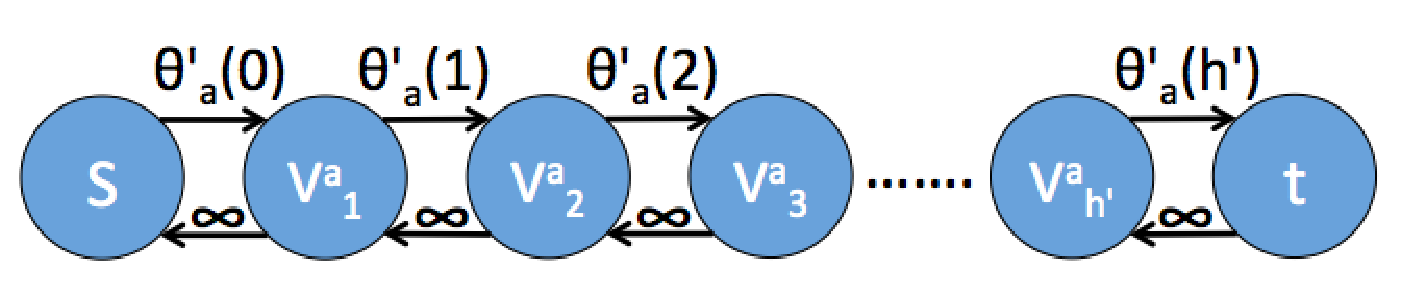
\psfig{file=\imagePath/theoryFig/unary_alt.eps,width=0.6\textwidth}
}
\vspace{3mm}
\mycaption{\footnotesize \em Arcs and their capacities for representing the unary potentials for the random variable $X_a$. According to the labeling defined
in equation~(\ref{eq:labeling}), if $x_a = \hat{x}_a$, then the arc $(s,V^a_1)$ will be cut, which will contribute exactly
$\theta_a(\hat{x}_a)$ to the capacity of the cut.
If $x_a = s+i-1$ where $i \in \{1,\cdots,h'-1\}$, then the arc $(V^a_i,V^a_{i+1})$ will be cut, which will contribute
exactly $\theta_a(s+i-1)$ to the capacity of the cut. If $x_a = l$, then the arc $(V^a_{h'},t)$ will be cut, which will contribute exactly
$\theta_a(l)$ to the capacity of the cut. The arcs with infinite capacity ensure that exactly one of the arcs from the set
$(s,V^a_1) \cup \{(V^a_i,V^a_{i+1}), i=1,\cdots,h'-1\} \cup (V^a_{h'},t)$ will be part of an $st$-cut with finite capacity,
which will guarantee that we are able to obtain a valid labeling.
}
\label{fig:unary}
\end{figure*}

\myparagraph{\bf Representing Unary Potentials.}
We will represent the unary potential
of $X_a$ using the arcs specified in Figure~\ref{fig:unary}. Since all the unary potentials are non-negative, it follows that the arc
capacities in Figure~\ref{fig:unary} are also non-negative.

\begin{figure*}[t]
\centering
\psfig{file=\imagePath/theoryFig/clique1.eps,width=0.30\textwidth}
\hspace{3cm}
\psfig{file=\imagePath/theoryFig/clique2.eps,width=0.30\textwidth}
\vspace{2mm}
\mycaption{\footnotesize \em Arcs used to represent the high-order potentials for the clique ${\bf X}_{\bf c} = \{X_1,X_2,\cdots,X_c\}$. {\bf Left.}
The term $r_{ij}$ is defined in equation~(\ref{eq:convexCapacity}). The arcs 
represent the sum of the $m$ maximum convex distance functions over disjoint pairs of random variables when no random variable retains
its old label. These arcs are specified only for $i \leq j$ and
when either one or both of $i$ and $j$ are not equal to 1. {\bf Right.} The terms $A$ and $B$ are defined in equation~(\ref{eq:submodCapacity}).
The arcs represent an overestimation of the clique potential for the case where some or all the random variables retain their old label.
}
\label{fig:clique}
\end{figure*}

\myparagraph{\bf Representing Clique Potentials.}
Consider a set of random variables ${\bf X}_{\bf c}$ that are used to define a high-order clique potential. Without loss of generality, we assume
${\bf X}_{\bf c} = \{X_1,X_2,\cdots,X_c\}$. In order to represent the potential value for a putative labeling ${\bf x}_{\bf c}$ of the clique, we
introduce two types of arcs, which are depicted in Figure~\ref{fig:clique}. For the arcs shown in Figure~\ref{fig:clique} (left), the capacities are
specified using the term $r_{ij}$ that is defined as follows:
\begin{equation}
\small r_{ij} = 
\begin{cases}
\omega_{\bf c}\frac{\overline{d}(i,j)}{2} & \text{if } i = j\\
\omega_{\bf c}\overline{d}(i,j)   & \text{otherwise.}
\end{cases}
\label{eq:convexCapacity}
\end{equation}
Here, the term $\overline{d}(i,j) = d(i-j+1) + d(i-j-1) - 2d(i-j) \geq 0$ since $d(\cdot)$ is convex, and
$\omega_{\bf c} \geq 0$ by definition. It follows that $r_{ij} \geq 0$ for all $i,j \in \{1,\cdots,h'\}$. 
For the arcs shown in Figure~\ref{fig:clique} (right), the capacities are specified using the terms $A$ and $B$ that are defined as follows:
\begin{equation}
\small A = \omega_{\bf c}M, B = \left(\omega_{\bf c}M-\frac{\theta_{\bf c}(\hat{\bf x}_{\bf c})}{m}\right).
\label{eq:submodCapacity}
\end{equation}
Since $M \geq 0$, and $\theta_{\bf c}(\hat{\bf x}_{\bf c}) \leq \omega_{\bf c}mM$ due to truncation, it follows that $A, B \geq 0$.


\subsubsection{Properties of the Graph}
\label{subsec:graph_properties}

This part describes the properties of the above graph construction which will facilitate the analysis of our algorithm for the truncated max-of-linear models.

\begin{property}The cost of the $st-$cut exactly represents the sum of the unary potentials associated with the corresponding labeling $f$, that is, $\sum_{v_a \in \bf_v} \theta_{a}(f(a))$.
\end{property}
This property follows from the description of the graph construction for unary potentials.
\begin{property} For $c \in \mathcal{C}$, if for all $X_a \in \mathbf{X_c}$, $f(a) = f_n(a) \notin I_n$ (all variables in a clique retain their old labels), then the cost of the $st-$cut exactly represents the clique potential plus a constant ${\bf \kappa}_{\bf c} = \omega_c m \cdot M - \theta_{\bf c}(\hat{{\bf x}_{\bf c}})$.
\end{property}
Graph (a) of figure~\ref{fig:clique} assigns $0$ cost. In graph (b), the vertices $\{V_1^1, \dots, V_1^c \} \in {\bf V}_{\bf t}$ and hence, the $s-U$ arc of capacity $mA$ is cut. 

\begin{align*}
mA &= \omega_c \cdot m \cdot M \\
&= \theta_{\bf c}(\hat{{\bf x}_{\bf c}}) + \omega_c m \cdot M - \theta_{\bf c}(\hat{{\bf x}_{\bf c}})\\
&= \theta_{\bf c}(\hat{{\bf x}_{\bf c}}) + {\bf \kappa}_{\bf c}
\end{align*}

\begin{property} If all variables in a clique move to a label in the current interval and $|l_c - l_1| \leq M$, then the cost of the $st-$cut exactly represents the clique potential plus a constant ${\bf \kappa}_{\bf c} = \omega_c m \cdot M - \theta_{\bf c}(\hat{{\bf x}_{\bf c}})$.
\end{property}

As proved in lemma~\ref{lemma:cliqueGraphProof}, graph (a) of figure~\ref{fig:clique} assigns exactly $\theta_{\bf c}({\bf x}_{\bf c})$ cost. In graph (b), the vertices $\{V_1^1, \dots, V_1^c \} \in {\bf V}_{\bf s}$ and hence, the $W-t$ arc of capacity $B$ is cut, where  

\begin{equation*}
B = \omega_c \cdot m \cdot M - \theta_{\bf c}(\hat{{\bf x}_{\bf c}}) = {\bf \kappa}_{\bf c}
\end{equation*}

\begin{property} If all variables in a clique move to a label in the current interval and $|l_c - l_1| \geq M$, then the cost of the $st-$cut overestimates the clique potential, being 

\begin{equation*}
\omega_c \sum_{i = 1}^{m} d(p_i({\bf x}_{\bf c} - p_{c - i + 1}({\bf x}_{\bf c})
\end{equation*}

plus a constant ${\bf \kappa}_{\bf c} = \omega_c m \cdot M - \theta_{\bf c}(\hat{{\bf x}_{\bf c}})$.

\end{property}

\begin{property} If $k ( < c)$ variables in a clique retains their old labels, then the cost of the $st-$cut overestimates the clique potential, being.
\end{property}

\begin{equation*}
\omega_c \sum_{i = 1}^{k} d(p_{c - i + 1}({\bf x}_{\bf c}) - i_n - 1) + \omega_c \cdot m \cdot M 
\end{equation*}

plus a constant ${\bf \kappa}_{\bf c} = \omega_c m \cdot M - \theta_{\bf c}(\hat{{\bf x}_{\bf c}})$.



\subsubsection{Proofs}

We first prove the following lemma, which will help us to establish properties of the graph:

\begin{lemma}
Graph (a) of figure~\ref{fig:clique} exactly models clique potentials that are proportional to the sum of $m$ maximum convex distance functions over all disjoint pairs of random variables of the clique.
\label{lemma:cliqueGraphProof}
\end{lemma}
Let us arrange the labels assigned to $\bf{X_c}$ in increasing order as $\{l_{k_{1}}, \dots ,l_{k_{c}}\}$, where $c = |\bf{X_c}|$ indicates the size of the clique. The sum of $m$ maximum convex distance functions over all disjoint pairs of random variables of the clique is given by:

\begin{equation}
\omega_{\bf c}(d(k_{c} - k_{1}) + d(k_{c-1} - k_{2}) + .... + d(k_{c-m+1} - k_{m}))
\end{equation}

When $i \in [k_{p} + 1, k_{p + 1}]$, exactly $p$ variables in ${\bf_{X_c}}$ are assigned a label between [$l_{k_{1}}$, $l_{k_{p}}$] and the corresponding $p$ vertices among $\{V^1_i, V^2_i....V^c_i\}$ will be in $\bf{V}_{t}$ (the remaining $c-t$ vertices will be in $\bf{V}_{s}$). Similarly, when $j \in [k_{c-p} + 1, k_{c-p+1}$], exactly $p$ variables in ${\bf_{X_c}}$ are assigned a label in the range [$l_{k_{c - p + 1}}$, $l_{k_{c}}$] and the corresponding $p$ vertices among $\{V^1_j, V^2_j....V^c_j\}$ will be in $\bf{V}_{s}$ (the remaining $c-p$ vertices will be in $\bf{V}_{t}$). $st$-{\sc mincut} includes either the arcs $(U_{ij}, V_{i}^{a})$ for all $V_{i}^{a} \in \bf{V}_{t}$ or the arcs $(V_{j}^{a}, W_{ij})$ for all $V_{j}^{a} \in \bf{V}_{s}$ or the arc $(W_{ij}, U_{ij})$, whichever contribute the smallest cost to the cut. Let $C_{ij}$ denote the sum of capacitites of arcs cut by $st$-{\sc mincut} in graph (a) of figure~\ref{fig:clique} for a given pair $i, j$. Clearly, $ 0 \leq C_{ij} \leq m \cdot r_{ij}$.

Let us partition the interval $[k_{1}+1, k_{c}]$ to $2m-1$ intervals $[k_{1}+1, k_{2}], [k_{2}+1, k_{3}],...[k_{m}+1, k_{c-m+1}]...,[k_{c-2}+1, k_{c-1}], [k_{c-1}+1, k_{c}] $. $C_{ij}$ depends on the intervals in which $i$ and $j$ lie. Given a labeling $\bf{x_{c}}$, the total contribution of all the cut arcs is equal to

\begin{align}
	\sum_{i=k_{1}+1}^{k_{c}} \sum_{j=i}^{k_{c}} C_{ij} &= \sum_{i=k_{1}+1}^{k_{2}} \sum_{j=i}^{k_{c}} C_{ij} +
\sum_{i=k_{2}+1}^{k_3} \sum_{j=i}^{k_{c}} C_{ij} \nonumber \\ &+\dotsb+  
\sum_{i=k_{m}+1}^{k_{c-m+1}} \sum_{j=i}^{k_{c}} C_{ij} +\dotsb+ \sum_{i=k_{c-1}+1}^{k_{c}} \sum_{j=i}^{k_{c}} C_{ij}
\label{eq:partition}
\end{align}

Consider the second term of the series in (\ref{eq:partition}). When $i \in [k_2 + 1, k_3]$, exactly 2 variables in ${\bf{X_c}}$ take up a label in the range $[k_1, k_2]$ and hence, two vertices among $\{V^1_i, V^2_i....V^c_i\}$ belong to $\bf{V}_{t}$. When $j \in [k_{c-1} + 1, k_c]$, only one vertex among $\{V^1_j, V^2_j....V^c_j\}$ belongs to $\bf{V}_{s}$, giving $C_{ij}$ as $r_{ij}$. For $j$ in all other intervals, at least two vertices among $\{V^1_j, V^2_j....V^c_j\}$ belong to $\bf{V}_{s}$, and $C_{ij}$ equals $2 \cdot r_{ij}$. Thus, the following holds


\begin{align*}
\sum_{i=k_{2}+1}^{k_3} \sum_{j=i}^{k_{c}} C_{ij} &= \sum_{i=k_{2}+1}^{k_3} \sum_{j=k_{c-1} + 1}^{k_{c}} r_{ij} + \sum_{i=k_{2}+1}^{k_3} \sum_{j=i}^{k_{c-1}} 2r_{ij} \\
&= \sum_{i=k_{2}+1}^{k_3} \sum_{j=k_{c-1} + 1}^{k_{c}} r_{ij} + \left(\sum_{i=k_{2}+1}^{k_3} \sum_{j=i}^{k_{c-1}} r_{ij} + \sum_{i=k_{2}+1}^{k_3} \sum_{j=i}^{k_{c-1}} r_{ij}\right)\\
&= \sum_{i=k_{2}+1}^{k_3} \sum_{j=i}^{k_{c}} r_{ij} + \sum_{i=k_{2}+1}^{k_3} \sum_{j=i}^{k_{c-1}} r_{ij}
\end{align*} 

where the last step is obtained by combining the first and the third terms in the summation.

In general, for $p \in [1, m-1]$ we can write

\begin{equation}
\sum_{i=k_{p}+1}^{k_{p+1}} \sum_{j=i}^{k_{c}} C_{ij} = \sum_{i=k_{p}+1}^{k_{p+1}} \sum_{j=i}^{k_{c}} r_{ij} + \sum_{i=k_{p}+1}^{k_{p+1}} \sum_{j=i}^{k_{c-1}} r_{ij} +\dotsb+ \sum_{i=k_{p}+1}^{k_{p+1}} \sum_{j=i}^{k_{c-p+1}} r_{ij}
\label{eq:regrouping}
\end{equation}

Similar argument can be extended for $p \in [c-m+1, c-1]$
 
\newpage
Using (\ref{eq:regrouping}), each term of (\ref{eq:partition}) can be written as

\begin{align*}
\sum_{i=k_{1}+1}^{k_{2}} \sum_{j=i}^{k_{c}} C_{ij} &= \sum_{i=k_{1}+1}^{k_{2}} \sum_{j=i}^{k_{c}} r_{ij}\\
\sum_{i=k_{2}+1}^{k_{3}} \sum_{j=i}^{k_{c}} C_{ij} &= \sum_{i=k_{2}+1}^{k_{3}} \sum_{j=i}^{k_{c}} r_{ij} + \sum_{i=k_{2}+1}^{k_{3}} \sum_{j=i}^{k_{c-1}} r_{ij}\\
\sum_{i=k_{3}+1}^{k_{4}} \sum_{j=i}^{k_{c}} C_{ij} &= \sum_{i=k_{3}+1}^{k_{4}} \sum_{j=i}^{k_{c}} r_{ij} + \sum_{i=k_{3}+1}^{k_{4}} \sum_{j=i}^{k_{c-1}} r_{ij} + \sum_{i=k_{3}+1}^{k_{4}} \sum_{j=i}^{k_{c-2}} r_{ij}\\
\vdots\\
\sum_{i=k_{m}+1}^{k_{c-m+1}} \sum_{j=i}^{k_{c}} C_{ij} &= \sum_{i=k_{m}+1}^{k_{c-m+1}} \sum_{j=i}^{k_{c}} r_{ij} + \sum_{i=k_{m}+1}^{k_{c-m+1}} \sum_{j=i}^{k_{c-1}} r_{ij} +\dotsb\dotsb+ \sum_{i=k_{m}+1}^{k_{c-m+1}} \sum_{j=i}^{k_{c-m+1}} r_{ij}\\
\vdots\\
\sum_{i=k_{c-3}+1}^{k_{c-2}} \sum_{j=i}^{k_{c}} C_{ij} &= \sum_{i=k_{c-3}+1}^{k_{c-2}} \sum_{j=i}^{k_{c}} r_{ij} + \sum_{i=k_{c-3}+1}^{k_{c-2}} \sum_{j=i}^{k_{c-1}} r_{ij} + \sum_{i=k_{c-3}+1}^{k_{c-2}} \sum_{j=i}^{k_{c-2}} r_{ij}\\
\sum_{i=k_{c-2}+1}^{k_{c-1}} \sum_{j=i}^{k_{c}} C_{ij} &= \sum_{i=k_{c-2}+1}^{k_{c-1}} \sum_{j=i}^{k_{c}} r_{ij} + \sum_{i=k_{c-2}+1}^{k_{c-1}} \sum_{j=i}^{k_{c-1}} r_{ij}\\
\sum_{i=k_{c-1}+1}^{k_{c}} \sum_{j=i}^{k_{c}} C_{ij} &= \sum_{i=k_{c-1}+1}^{k_{c}} \sum_{j=i}^{k_{c}} r_{ij}
\end{align*}
Adding all the above equations by adding all terms vertically, we obtain
\begin{align*}
\sum_{i=k_{1}+1}^{k_{c}} \sum_{j=i}^{k_{c}} C_{ij} &= \sum_{i=k_{1}+1}^{k_{c}} \sum_{j=i}^{k_{c}} r_{ij} +
\sum_{i=k_{2}+1}^{k_{c-1}} \sum_{j=i}^{k_{c-1}} r_{ij} +\dotsb+ 
\sum_{i=k_{m}+1}^{k_{c-m+1}} \sum_{j=i}^{k_{c-m+1}} r_{ij}\\\\
&= \omega_{\bf{c}}d(k_{c}-k_{1}) + \omega_{\bf{c}}d(k_{c-1}-k_{2}) +\dotsb+
\omega_{\bf{c}}d(k_{c-m+1}-k_{m})
\end{align*}

Hence, graph (a) of figure~\ref{fig:clique} represents exactly clique potentials that are proportional to the sum of $m$ maximum convex distance functions over all disjoint pairs of random variables of the clique. \hspace{6mm} $\blacksquare$

The following proposition follows from the properties of the graph described in subsection~\ref{subsec:graph_properties}:

\begin{proposition}
\label{prop:graphCut}
Given a cut that partitions the vertices ${\bf V}$ into two disjoint sets ${\bf V}_s$ and ${\bf V}_t$, and the corresponding
labeling ${\bf y}$, the capacity of the cut is equal to the energy $E'({\bf y})$
up to a constant.
\end{proposition}

\paragraph{Energy Minimization.} The above proposition implies that 
the labeling ${\bf y}'$ that corresponds to the $st$-{\sc mincut} minimizes the energy $E'(\cdot)$ over all
possible labelings ${\bf y} \in ({\bf L}')^n$. Since all the arc capacities of the directed graph are non-negative, it follows that
the labeling ${\bf y}'$ can be computed efficiently by solving the $st$-{\sc mincut} problem on the directed graph defined above.
Once the labeling ${\bf y}'$ is computed, the approximate solution to problem~(\ref{eq:rangeMove}) can be computed as follows:
\begin{equation}
x'_a = 
\begin{cases}
\hat{x}_a & \text{if } y'_a = 0, \\
y'_a+f & \text{otherwise.}
\end{cases}
\end{equation}
This completes our description of the range expansion algorithm. In section~\ref{sec:Bounds}, we establish its theoretical guarantees for
some interesting special cases.

%Recall that a convex distance function satisfies the following properties: (i) $d(y) \geq 0$ for all $y \in \mathbb{Z}$ and $d(0) = 0$;
%(ii) $d(y) = d(-y)$ for all $y \in \mathbb{Z}$; and (iii) $d(y+1)-2d(y)+d(y-1) \geq 0$ for
%all $y \in \mathbb{Z}$. The above properties also imply that $d(y) \geq d(z)$ if $|y| \geq |z|$, for all $y,z \in \mathbb{Z}$.

\section{Multiplicative Bounds}
\label{sec:Bounds}


\subsection{Bounds for Truncated Max-of-linear Models}

Let $f_n$ denote the labeling after the $n$-th iteration and $E(f_n)$ denote the corresponding energy. Also, $f^*$ denotes optimal labeling of the MRF.

Let $r \in [0, L-1]$ be a uniformly distributed random integer and $L$ be the length of the interval. Using $r$ we define the following set of intervals
\begin{equation*}
	\Gamma_r = \left\{[0, r], [r + 1, r + L], [r + L + 1, r + 2L], ..., [., h -1]\right\}
\end{equation*}
where $h$ is the total number of labels.

Let \textbf{X}$(f^*, I_{n})$ contain all the random variables that take an optimal labeling in $I_{n}$, $\mathcal{A}\mathit(f, I_n)$ be the set of all cliques for which all variables take optimum label in the interval $I_{n}$ and $\mathcal{B}\mathit(f, I_n)$ be the set of all cliques for which at least one, but not all, variable takes optimum label in the interval $I_{n}$ (that is, at least one but not all variables retains old label).

In order to make the analysis more readable, the following shorthand notation is introduced:

\begin{itemize}
	\item We denote $\mathbf{\omega_c} \max_{a, b \in \mathbf{X_c}} d(f^*(a) - f^*(b))$ as $t_c^n$
	\item We denote $\mathbf{\omega_c} \max_{a \in \mathbf{X_c}} d(f^*(a) - (i_n + 1)) + \mathbf{\omega_c}\mathit{M} $ as $s_c^n$
\end{itemize}

We now define two lemmas which we will make use of later:

\begin{lemma}
At an iteration of our algorithm, given the current labeling $f_n$ and an interval $I_n = [i_n + 1, j_n]$, the new labeling $f_{n+1}$ obtained by solving the st-mincut problem reduces the energy by at least the following:

\begin{equation*}
	\begin{split}
		& \sum_{X_a \in {\bf X}(f^*, I_{n})} \theta_{a}(f_n(a)) + \sum_{{\bf X_c} \in \mathcal{A}\mathit(f, I_n) \cup \mathcal{B}\mathit(f, I_n)} \theta_{\bf c}({\bf x_c}) \\
		&	  - \left( \sum_{X_a \in {\bf X}(f^*, I_{n})} \theta_{a}(f^*(a)) + \sum_{{\bf X_c} \in \mathcal{A}\mathit(f, I_n)} t_c^n 
	 +  \sum_{{\bf X_c} \in \mathcal{B}\mathit(f, I_n)} s_c^n \right) 
	 \end{split}
\end{equation*}
\label{lemma:reductionlowerBound}
\end{lemma}

It is evident from the properties of the graph discussed in subsection~\ref{subsec:graph_properties} that the energy of the new labeling $f_{n+1}$ is bounded from above by the cost of the $st$-mincut. The cost of the $st$-mincut itself is bounded from above by the cost of any other $st$-cut in the graph. Consider one such $st$-cut that gives the following labeling:

\begin{align*}
 f(a) = 
	\begin{cases}
		f^*(a) & if \hspace{2mm} X_a \in \mathbf{X}(f^*, I_n) \\
		f_n(a) & otherwise.
	\end{cases}
\end{align*}

We can derive the cost of this $st$-cut using the properties of subsection~\ref{subsec:graph_properties}. The energy of $f$ equals the sum of the terms in the properties minus $\sum_{c \in \mathcal{C}} \kappa_{c}$. The energy of $f_{n+1}$ is less than that of $f$. Hence, the difference between the energy of the current labeling $f_n$ and the new labeling $f_{n+1}$, i.e $E(f_n) - E(f_{n+1})$, is at least

\begin{align*}
	\begin{split}
		& \sum_{X_a \in {\bf X}(f^*, I_{n})} \theta_{a}(f_n(a)) + \sum_{{\bf X_c} \in \mathcal{A}\mathit(f, I_n) \cup \mathcal{B}\mathit(f, I_n)} \theta_{\bf c}({\bf x_c}) \\
		&	  - \left( \sum_{X_a \in {\bf X}(f^*, I_{n})} \theta_{a}(f^*(a)) + \sum_{{\bf X_c} \in \mathcal{A}\mathit(f, I_n)} t_c^n 
	 +  \sum_{{\bf X_c} \in \mathcal{B}\mathit(f, I_n)} s_c^n \right) 
	 \end{split}
 \end{align*}

 This proves the lemma. \hspace{6mm} $\blacksquare$ 
\begin{lemma}
When $d(.)$ is linear, that is, $d(x) = |x|$, the following inequality holds true:
\begin{equation}
\begin{split}
& \frac{1}{L}\sum_{r}\sum_{I_n \in \Gamma_r}\left(\sum_{{\bf X_c} \in \mathcal{A}\mathit(f, I_n)} t_c^n + \sum_{{\bf X_c} \in \mathcal{B}\mathit(f, I_n)} s_c^n \right) \\
& \leq  max \left\{ \frac{c}{2}\left(2 + \frac{L}{M}\right), \left(2 + \frac{2M}{L}\right) \right\} \sum_{{\bf c} \in \mathcal{C}} \theta_{\bf c}(\bf {x_c})
\end{split}
\end{equation}
where $\mathit{c}$ is the largest clique in the random field.
\label{lemma:linearIneq}
\end{lemma}

Let us denote the set of optimum labels in a clique $\mathbf{X_{c}}$ arranged in an increasing order as ${l_1, l_2....., l_{c-1}, l_c}$. Since we are dealing with the truncated linear metric, the terms $t_c^n$ and $s_c^n$ can be simplified as:

\begin{equation}
	t_c^n = \omega_c (l_c - l_1), s_c^n = \omega_c (l_c - i_n - 1 + M)
\end{equation}

The LHS of inequality in lemma \ref{lemma:linearIneq} can be written as:

\begin{equation}
\frac{1}{L}\sum_{{\bf c} \in \mathcal{C}}\left(\sum_{\mathcal{A}\mathit(f, I_n) \ni {\bf c}} t_c^n + \sum_{\mathcal{B}\mathit(f, I_n) \ni {\bf c}} s_c^n \right)
\label{eq:rewriteIneq}
\end{equation}

In order to prove the lemma, we consider the following three cases for each clique ${\bf X_c}$: \\

$Case - I: |l_c - l_1| \geq L$ and hence $\theta_{\bf c}(\bf{x_c}) = \omega_c \cdot M$

In this case, ${\bf X_c} \notin \mathcal{A}\mathit(f, I_n)$ for all intervals $I_n$ since the length of each interval is $L$. Moreover, the conditions for ${\bf X_c} \in \mathcal{B}\mathit(f, I_n)$ are given by

\begin{equation*}
	{\bf X_c} \in \mathcal{B}\mathit(f, I_n) \iff i_n \in [l_1 - L, l_c - 1]
\end{equation*}
We observe that

\begin{align}
	& \sum_{\mathcal{A}\mathit(f, I_n) \ni {\bf c}} t_c^n + \sum_{\mathcal{B}\mathit(f, I_n) \ni {\bf c}} s_c^n \nonumber\\
	\leq{}  & \omega_c \sum_{p = 1}^{c} \sum_{l_p - L}^{l_p - 1} \left( M + l_p - i_n - 1 \right)\nonumber\\        
	={}  & \omega_c \sum_{p=1}^{c} \left(L \cdot M + \frac{L \cdot (L - 1)}{2}\right) \nonumber\\
	={}  & L \cdot \frac{c}{2} \left( 2 + \frac{L - 1}{M} \right) \theta_{\bf c}(\bf{x_c}) \nonumber\\
	\leq{}  & L \cdot \frac{c}{2} \left( 2 + \frac{L}{M} \right) \theta_{\bf c}(\bf{x_c}) \label{eq:case1bound}
\end{align}
	
$Case - II: M \leq |l_c - l_1| < L$ and hence $\theta_{\bf c}(\bf{x_c}) = \omega_c \cdot M$

In this case, the conditions for ${\bf X_c} \in \mathcal{A}\mathit(f, I_n)$ and $X_c \in \mathcal{B}\mathit(f, I_n)$ are given by

\begin{align*}
& {\bf X_c} \in \mathcal{A}\mathit(f, I_n) \iff i_n \in [l_c - L, l_1 - 1] \\
& {\bf X_c} \in \mathcal{B}\mathit(f, I_n) \iff i_n \in [l_1 - L, l_c - L - 1] \cup [l_1, l_c - 1]\\
\end{align*}
We observe that

\begin{align*}
	& \sum_{\mathcal{A}\mathit(f, I_n) \ni {\bf c}} t_c^n + \sum_{\mathcal{B}\mathit(f, I_n) \ni {\bf c}} s_c^n \\
	={}  & \omega_c \left( \sum_{i_n = l_c - L}^{l_1 - 1} (l_c - l_1) + \left\{ \sum_{p = 1}^{c-1} \sum_{i_n = l_p - L}^{l_{p+1}-L-1} (M + l_p - (i_n + 1)) \right.\right.\\ 
	     & \left. \left. + \sum_{i_n = l_1}^{l_c -1} (M + l_c - (i_n + 1)) \right\}\right)\\        
	={} & \omega_c \left( A + B + C \right) \\
\end{align*}
where
\begin{align*}
	A  ={} &\sum_{i_n = l_c - L}^{l_1 - 1} (l_c - l_1) \\
	B  ={} &\sum_{p = 1}^{c-1} \sum_{i_n = l_p - L}^{l_{(p+1)}-L-1} (M + l_p - (i_n + 1)) \\
	C  ={} &\sum_{i_n = l_1}^{l_c -1} (M + l_c - (i_n + 1)) \\
\end{align*}
Let $(l_c - l_1) = r$. Hence, we have:

\begin{align}
	A & = (l_c - l_1)\cdot(L - (l_c - l_1)) \nonumber\\
	  & = r \cdot (L - r) = L \cdot r - r^2 \label{eq:Aexpr}
\end{align}

\begin{align*}
	& B = \sum_{p = 1}^{c-1} \sum_{i_n = l_p - L}^{l_{(p+1)}-L-1} (M + l_p - (i_n + 1)) \\
	&  = \sum_{p = 1}^{c-1} \sum_{i_n = l_p - L}^{l_{(p+1)}-L-1} M + \\
	& \sum_{p = 1}^{c-1} \sum_{i_n = l_p - L}^{l_{(p+1)}-L-1} (l_p - (i_n + 1)) \\
	& = \sum_{p = 1}^{c-1} M \cdot (l_{(p+1)} - l_p) +  \\
	& \sum_{p = 1}^{c-1}\left\{(L-1) +.....+ (L-(l_{p+1}-l_p))\right\} \\
\end{align*}

Let $ y_p = l_{(p+1)} - l_p $. Clearly 
\begin{equation*}
\sum_{p=1}^{c-1} y_p = l_c - l_1 \\
\end{equation*}	

Hence,

\begin{align}
 B & = M \cdot r + L \cdot r - \sum_{p=1}^{c-1} \frac{y_p \cdot (y_p + 1)}{2} \nonumber \\
	  & = M \cdot r + L \cdot r - \frac{r}{2} - \sum_{p=1}^{c-1} \frac{(y_p)^2}{2} \label{eq:Bexpr}
\end{align}

\begin{align}
	C & = \sum_{i_n = l_1}^{l_c - 1} (M + l_c - (i_n + 1)) \nonumber\\
	  & = \sum_{i_n = l_1}^{l_c - 1} M + \sum_{i_n = l_1}^{l_c - 1} \left(l_c - (i_n + 1) \right) \nonumber\\
	  & = M\cdot(l_c - l_1) + \left\{ (l_c - (l_1 + 1)) + (l_c - (l_1 + 2))... + 1 \right\} \nonumber \\
	& = M\cdot(l_c - l_1) + \frac{(l_c - l_1 - 1)(l_c - l_1)}{2} \nonumber \\
	& = M \cdot r + \frac{(r-1)\cdot r}{2} \nonumber \\
	& = M \cdot r + \frac{r^2}{2} - \frac{r}{2} \label{eq:Cexpr}
\end{align}

Using \eqref{eq:Aexpr}, \eqref{eq:Bexpr}, \eqref{eq:Cexpr}, we have

\begin {equation} \label{eq:sum_ABC}
A + B + C = (2L + 2M - r)r + \frac{r^2}{2} - r -\sum_{p=1}^{c-1}\frac{y_{p}^2}{2}
\end{equation}

We have
\begin{equation*}
	\sum_{p = 1}^{c-1} \frac{{y_p}^2}{2} \geq \frac{r^2}{2(c-1)} \\
\end{equation*}
(Taking each $y_p = r/(c-1)$)

%The following expression can be simplified:
%\begin{align*}
%	\frac{r^2}{2} - r - \frac{r^2}{2(c-1)^2}
%	= \left\{\frac{r \cdot c \cdot (c-2)}{2(c-1)^2} - 1 \right\} \cdot r
%\end{align*}

Hence,

\begin{equation*}
	A + B + C \leq \left\{2L + 2M - 1 - \frac{r}{2}\left(\frac{c}{c - 1}\right)\right\}\cdot r
\end{equation*}

Let 

\begin{equation*}
	f(r) = \left\{2L + 2M - 1 - \frac{r}{2} \left(\frac{c}{c - 1}\right)\right\}\cdot r
\end{equation*}

Taking derivative of $f(r)$, we obtain

\begin{equation*}
	f'(r) = 2L + 2M - 1 - \frac{r \cdot c}{(c-1)} 
\end{equation*}

$f(r)$ is a quadratic function which opens downwards (coefficient of $r^2$ is negative). Also

\begin{equation*}
	f'(L) = \left(\frac{c - 2}{c - 1}\right) \cdot L + 2M - 1 > 0 
\end{equation*}

Hence, using $r = L$,

\begin{align}
A + B + C & < L \cdot \left\{2L + 2M - 1 - \frac{L}{2} \cdot \left( \frac{c}{c - 1} \right) \right\} \nonumber\\
			       & < L \cdot \left\{\frac{2L}{M} + 2 - \frac{L}{2M} \cdot \left( \frac{c}{c - 1} \right) \right\} \theta_{\bf c}(\bf{x_c}) \label{eq:case2bound}
\end{align}
where the last expression is obtained using the fact that $\theta_{\bf c}(\bf{x_c}) = \omega_c \cdot M$. \\


$Case - III: |l_c - l_1| < M$ and hence $\theta_{\bf c}(\bf{x_c}) = \omega_c(l_c - l_1)$

In this case, the conditions for ${\bf X_c} \in \mathcal{A}\mathit(f, I_n)$ and ${\bf X_c} \in \mathcal{B}\mathit(f, I_n)$ are given by

\begin{align*}
& {\bf X_c} \in \mathcal{A}\mathit(f, I_n) \iff i_n \in [l_c - L, l_1 - 1] \\
& {\bf X_c} \in \mathcal{B}\mathit(f, I_n) \iff i_n \in [l_1 - L, l_c - L - 1] \cup [l_1, l_c - 1]\\
\end{align*}

We observe that

\begin{align*}
	& \sum_{\mathcal{A}\mathit(f, I_n) \ni {\bf c}} t_c^n + \sum_{\mathcal{B}\mathit(f, I_n) \ni {\bf c}} s_c^n \\
	={}  & \omega_c \left( \sum_{i_n = l_c - L}^{l_1 - 1} (l_c - l_1) + \left\{ \sum_{p = 1}^{c-1} \sum_{i_n = l_p - L}^{l_{p+1}-L-1} (M + l_p - (i_n + 1)) \right.\right.\\ 
	     & \left. \left. + \sum_{i_n = l_1}^{l_c -1} (M + l_c - (i_n + 1)) \right\}\right)\\        
	={} & \omega_c \left( A + B + C \right) \\
\end{align*}

Similar to case II, we can write

\begin{equation*} \label{eq:rewrite_sum_ABC}
A + B + C = (2L + 2M - r/2)r - r -\sum_{p=1}^{c-1}\frac{y_{p}^2}{2} \\
\end{equation*}

Since $r < M$

\begin{align}
	A + B + C &\leq (2L + 2M)(l_{c} - l_{1}) \nonumber\\
		  & = L\left(2 + \frac{2M}{L}\right) \theta_{\bf c}(\bf{x_c}) \label{eq:case3bound}
\end{align}
where the last expression is obtained using the fact that $\theta_{\bf c}(\bf{x_c}) = \omega_c \cdot M$.

Substituting inequalities \eqref{eq:case1bound}, \eqref{eq:case2bound} and \eqref{eq:case3bound} in expression \eqref{eq:rewriteIneq} and dividing both sides by $L$ for all $\bf{X_c}$, we obtain inequality of lemma \ref{lemma:linearIneq}. This proves the lemma. \hspace{6mm} $\blacksquare$ 


\begin{proposition}
\label{prop:linearBound}
The range expansion algorithm with $h' = M$ has a multiplicative bound of $O(C)$ for truncated max-of-linear model when $m=1$. The
term $C$ equals the size of the largest clique. Hence, if ${\bf x}^*$ is a labeling with
minimum energy and $\hat{\bf x}$ is the labeling estimated by range expansion algorithm then
\begin{equation}
\small
\sum_{a \in {\cal V}} \theta_a(\hat{x}_a) + \sum_{{\bf c} \in {\cal C}} \theta_{\bf c}(\hat{\bf x}_{\bf c}) \leq \nonumber 
\sum_{a \in {\cal V}} \theta_a({x}^*_a) + O(C) \sum_{{\bf c} \in {\cal C}} \theta_{\bf c}({\bf x}^*_{\bf c}).
\label{eq:linear_bound}
\end{equation}
The above inequality holds for arbitrary set of unary potentials and non-negative clique weights.
\end{proposition}

The following equation can be deduced from the above definitions:

\begin{equation} \label{unary_sum}
	\sum_{X_a \in \mathbf{X}} \theta_a(f^*(a)) = \sum_{I_n \in \mathcal{I}_r} \sum_{X_a \in \mathbf{X}(f^*, I_{n})} \theta_{a}(f^*(a))
\end{equation}

since $f^*(a)$ belongs to exactly one interval in $I_r$ for all $X_a$. 

For the final labeling $f$ of the range expansion algorithm, the term in lemma~\ref{lemma:reductionlowerBound} should be non-positive for all intervals $I_n$ because $f$ is a local optimum. Hence,

\begin{equation*}
	\begin{split}
		&\sum_{X_a \in {\bf X}(f^*, I_{n})} \theta_{a}(f(a)) + \sum_{{\bf X_c} \in \mathcal{A}\mathit(f, I_n) \cup \mathcal{B}\mathit(f, I_n)} \theta_{\bf c}({\bf x_c})\\
	 & \leq \left( \sum_{X_a \in {\bf X}(f^*, I_{n})} \theta_{a}(f^*(a)) + \sum_{{\bf X_c} \in \mathcal{A}\mathit(f, I_n)} t_c^n 
	 +  \sum_{{\bf X_c} \in \mathcal{B}\mathit(f, I_n)} s_c^n \right), \forall I_{n} 
	\end{split}
\end{equation*}

We sum the above inequality over all $I_n \in \Gamma_r$. The summation of the LHS is at least $E(f)$. Also, using \eqref{unary_sum}, the summation of the above inequality can be written as:

\begin{equation*}
E(f) \leq \sum_{X_a \in {\bf X}} \theta_{a}(f^*(a)) + \sum_{I_n \in \Gamma_r}\left(\sum_{{\bf X_c} \in \mathcal{A}\mathit(f, I_n)} t_c^n + \sum_{{\bf X_c} \in \mathcal{B}\mathit(f, I_n)} s_c^n \right)
\end{equation*}

We now take the expectation of the above inequality over the uniformly distributed random integer $r \in [0, L - 1]$. The LHS of the inequality and the first term on the RHS (that is, $\sum \theta_a(f^*(a)))$ are constants with respect to $r$. Hence, we get

\begin{equation}
E(f) \leq \sum_{X_a \in {\bf X}} \theta_{a}(f^*(a)) + \frac{1}{L}\sum_{r}\sum_{I_n \in \Gamma_r}\left(\sum_{{\bf X_c} \in \mathcal{A}\mathit(f, I_n)} t_c^n + \sum_{{\bf X_c} \in \mathcal{B}\mathit(f, I_n)} s_c^n \right)
\label{eq:upperboundfinalenergy}
\end{equation} 

Lemma~\ref{lemma:linearIneq} allows us to write the above inequality as 

\begin{equation}
E(f) \leq \sum_{X_a \in {\bf X}} \theta_{a}(f^*(a)) + max \left\{ \frac{c}{2}\left(2 + \frac{L}{M}\right), \left(2 + \frac{2M}{L}\right) \right\} \sum_{{\bf c} \in \mathcal{C}} \theta_{\bf c}(\bf {x_c})
\end{equation}

The R.H.S of lemma \ref{lemma:linearIneq} is minimum under the following condition:

\begin{equation}
\label{eq:linearboundEquality}
\frac{c}{2}\left(2 + \frac{L}{M}\right) =  \left(2 + \frac{2M}{L}\right)
\end{equation}
The positive solution of the above quadratic equation gives the optimum value $L_{opt}$ of interval length:

\begin{equation}
	L_{opt} = \left\{\frac{2 - c + \sqrt{c^2 + 4}}{c}\right\}\cdot M
\label{eq:Loptimum}
\end{equation}

However, we bound the minimum value of L as M, giving:

\begin{equation}
	L_{opt} = max\left\{\left\{\frac{2 - c + \sqrt{c^2 + 4}}{c}\right\}\cdot M, M\right\}
\label{eq:Loptimumbound}
\end{equation}

Note $L_{opt}$ equals $\sqrt{2}M$ for $c = 2$ and $M$ for $c > 2$. Substituting the optimum value of L from equation \ref{eq:Loptimumbound} in inequality of lemma \ref{lemma:linearIneq} and simplifying inequality \ref{eq:upperboundfinalenergy} gives the multiplicative bound for truncated max-of-linear model as $\frac{(c+2) + \sqrt{c^2 + 4}}{2}$. Hence, the multiplicative bound is $O(c)$ where $c$ is the size of the maximal clique. For $c = 2$, this gives a bound of 2 + $\sqrt{2}$ using $L = \sqrt{2}M$. \hspace{6mm} $\blacksquare$ 

\vspace{4mm}

\subsection{Bounds for $m$-Truncated Max-of-linear Models}

We will now give the multiplicative bound of our range expansion algorithm for $m$-max-of-linear for any value of $m$. 

We need some definitions before we analyse the bound. Let $\mathcal{A}\mathit(f, I_n)$ be the set of all cliques for which all variables take optimum label in the interval $I_{n}$ and $\mathcal{B}_k\mathit(f, I_n)$ where $k \in [1, \dots, m -1]$ be the set of all cliques for which exactly $k$ variables retain their old label. Let $\mathcal{B}_m\mathit(f, I_n)$ be the set of all cliques for which $m$ or more variables retain their old label.

We also introduce the following shorthand notation:

\begin{itemize}
	\item We denote $\mathbf{\omega_c}\{\sum_{i = 1}^{m} d(p_i({\bf x}_c) - p_{c - i + 1}({\bf x}_c)\} $ as $t_{m, c}^n$
	\item We denote $\mathbf{\omega_c}\{\sum_{i = 2}^{m - 1} d(p_i({\bf x}_c) - p_{c - i + 1}({\bf x}_c) +  d(p_{c}({\bf x}_c) - i_m - 1) \} +  \mathbf{\omega_c}\cdot M$ as $s_{1, c}^n$
	\item In general, we denote $\mathbf{\omega_c}\{\sum_{i = k + 1}^{m - k} d(p_i({\bf x}_c) - p_{c - i + 1}({\bf x}_c) + \sum_{i = 1}^{k} d(p_{c - i + 1}({\bf x}_c) - i_m - 1) \} + $k$ \cdot  \mathbf{\omega_c}\cdot M$ as $s_{k, c}^n$
\end{itemize}

We state the following lemma which is a generalization of lemma~\ref{lemma:reductionlowerBound}.

\begin{lemma}
At an iteration of our algorithm, given the current labeling $f_n$ and an interval $I_n = [i_n + 1, j_n]$, the new labeling $f_{n+1}$ obtained by solving the st-mincut problem reduces the energy by at least the following:

\begin{equation*}
	\begin{split}
		& \sum_{X_a \in {\bf X}(f^*, I_{n})} \theta_{a}(f_n(a)) + \sum_{{\bf X_c} \in \mathcal{A}\mathit(f, I_n) \cup \mathcal{B}_1\mathit(f, I_n) \cup \dots  \cup \mathcal{B}_m\mathit(f, I_n)} \theta_{\bf c}({\bf x_c}) \\
		&	  - \left( \sum_{X_a \in {\bf X}(f^*, I_{n})} \theta_{a}(f^*(a)) + \sum_{{\bf X_c} \in \mathcal{A}\mathit(f, I_n)} t_{m, c}^n 
	 +  \sum_{{\bf X_c} \in \mathcal{B}_1\mathit(f, I_n)} s_{1, c}^n +  \dots + \sum_{{\bf X_c} \in \mathcal{B}_m\mathit(f, I_n)} s_{m, c}^n \right) 
	 \end{split}
\end{equation*}
\label{lemma:mreductionlowerBound}
\end{lemma}

We also make use of the following lemma which generalizes lemma~\ref{lemma:linearIneq}:

\begin{lemma}
When $d(.)$ is linear, that is, $d(x) = |x|$, the following inequality holds true:
\begin{equation}
\begin{split}
& \frac{1}{L}\sum_{r}\sum_{I_n \in \Gamma_r}\left(\sum_{{\bf X_c} \in \mathcal{A}\mathit(f, I_n)} t_{m, c}^n +  \sum_{{\bf X_c} \in \mathcal{B}_1\mathit(f, I_n)} s_{1, c}^n +  \dots + \sum_{{\bf X_c} \in \mathcal{B}_m\mathit(f, I_n)} s_{m, c}^n \right) \\
& \leq  max \left\{ m \cdot \frac{c}{2}\left(2 + \frac{L}{M}\right), \left(2 + \frac{2M}{L}\right) \right\} \sum_{{\bf c} \in \mathcal{C}} \theta_{\bf c}(\bf {x_c})
\end{split}
\end{equation}
where $\mathit{c}$ is the largest clique in the random field.
\label{lemma:mlinearIneq}
\end{lemma}

Let us denote the set of optimum labels in a clique $\mathbf{X_{c}}$ arranged in an increasing order as ${l_1, l_2....., l_{c-1}, l_c}$. Since we are dealing with the truncated linear metric, the terms $t_{m, c}^n$ and $s_{k, c}^n$ can be simplified as:

\begin{align*}
t_{m, c}^n & = {\bf \omega}_{c}\{(l_c - l_1) + (l_{c - 1} - l_2) + \dots + (l_{c - m + 1} - l_m)\} \\
s_{1, c}^n & = {\bf \omega}_{c}\{(l_c - i_n - 1 + M) + (l_{c - 1} - l_2) + \dots + (l_{c - n + 1}- l_n)\}\\
\vdots \\
s_{m, c}^n & = {\bf \omega}_{c}\{(l_c - i_n - 1 + M) + (l_{c - 1} - i_n - 1 + M) + \dots + (l_{c - n + 1}- i_n - 1 + M)\}\\
\end{align*}

Since the labels are sorted in ascending order $\{l_1, \dots , l_c \}$, it follows that
\begin{align*}
t_{m, c}^n & \leq {\bf \omega}_{c} \cdot m \cdot \{l_c - l_1 \} \\
s_{1, c}^n & \leq {\bf \omega}_{c} \cdot m \cdot \{l_c - i_n - 1 + M\} \\ 
\vdots \\
s_{m, c}^n & \leq {\bf \omega}_{c} \cdot m \cdot \{l_c - i_n - 1 + M\} \\ 
\end{align*}

The LHS of inequality in lemma \ref{lemma:mlinearIneq} can be written as:

\begin{equation}
\begin{split}
& \frac{1}{L}\sum_{{\bf c} \in \mathcal{C}}\left(\sum_{\mathcal{A}\mathit(f, I_n) \ni {\bf c}} t_{m, c}^n + \sum_{\mathcal{B}_1 \mathit(f, I_n) \ni {\bf c}} s_{1, c}^n + \dots + \sum_{\mathcal{B}_m \mathit(f, I_n) \ni {\bf c}} s_{m, c}^n \right) \\
& \leq \frac{1}{L}\sum_{{\bf c} \in \mathcal{C}}\left(\sum_{\mathcal{A}\mathit(f, I_n) \ni {\bf c}} {\bf \omega}_{c} \cdot m \cdot \{l_c - l_1 \} + \sum_{\mathcal{B}_1 \mathit(f, I_n) \ni {\bf c}} {\bf \omega}_{c} \cdot m \cdot \{l_c - i_n - 1 + M\} + \dots \right. \\
&\left. + \sum_{\mathcal{B}_m \mathit(f, I_n) \ni {\bf c}} {\bf \omega}_{c} \cdot m \cdot \{l_c - i_n - 1 + M\}\right) \\
& \leq \frac{1}{L}\sum_{{\bf c} \in \mathcal{C}}\left(\sum_{\mathcal{A}\mathit(f, I_n) \ni {\bf c}} {\bf \omega}_{c} \cdot m \cdot \{l_c - l_1 \} + \sum_{\mathcal{B}_1 \mathit(f, I_n) \cup \dots \cup \mathcal{B}_m \mathit(f, I_n) \ni {\bf c}} {\bf \omega}_{c} \cdot m \cdot \{l_c - i_n - 1 + M\} \right) \\
& = m \cdot \frac{1}{L}\sum_{{\bf c} \in \mathcal{C}}\left(\sum_{\mathcal{A}\mathit(f, I_n) \ni {\bf c}} {\bf \omega}_{c} \cdot t_c^n + \sum_{\mathcal{B} \mathit(f, I_n) \ni {\bf c}} {\bf \omega}_{c} \cdot s_c^n \right) \\
\label{eq:mrewriteIneq}
\end{split}
\end{equation}

The last expression in equation~\ref{eq:mrewriteIneq} is $m$ times expression~\ref{eq:rewriteIneq}. The analysis below follows the same steps as in lemma~\ref{lemma:linearIneq}.

In order to prove the lemma, we consider the following three cases for each clique ${\bf X_c}$: \\

$Case - I: |l_c - l_1| \geq L$ and hence $ \omega_c \cdot M \leq \theta_{\bf c}({\bf{x_c}}) \leq \omega_c \cdot m \cdot M$

This results in 

\begin{align}
m \cdot \frac{1}{L}\sum_{{\bf c} \in \mathcal{C}}\left(\sum_{\mathcal{A}\mathit(f, I_n) \ni {\bf c}} {\bf \omega}_{c} \cdot t_c^n + \sum_{\mathcal{B} \mathit(f, I_n) \ni {\bf c}} {\bf \omega}_{c} \cdot s_c^n \right) &\leq m \cdot \frac{c}{2} \left( 2 + \frac{L}{M} \right) \omega_c \cdot M \nonumber \\
& \leq m \cdot \frac{c}{2} \left( 2 + \frac{L}{M} \right) \theta_{\bf c}({\bf{x_c}})
\label{eq:mcase1bound}
\end{align}

$Case - II: M \leq |l_c - l_1| < L$ and hence $ \omega_c \cdot M \leq \theta_{\bf c}({\bf{x_c}}) \leq \omega_c \cdot m \cdot M$

This gives

\begin{align}
m \cdot \frac{1}{L}\sum_{{\bf c} \in \mathcal{C}}\left(\sum_{\mathcal{A}\mathit(f, I_n) \ni {\bf c}} {\bf \omega}_{c} \cdot t_c^n + \sum_{\mathcal{B} \mathit(f, I_n) \ni {\bf c}} {\bf \omega}_{c} \cdot s_c^n \right) &\leq
m \cdot \left\{\frac{2L}{M} + 2 - \frac{L}{2M} \cdot \left( \frac{c}{c - 1} \right) \right\} \omega_c \cdot M \nonumber \\
& \leq m \cdot \left\{\frac{2L}{M} + 2 - \frac{L}{2M} \cdot \left( \frac{c}{c - 1} \right) \right\}  \theta_{\bf c}({\bf{x_c}})
\label{eq:mcase2bound}
\end{align}

$Case - III: |l_c - l_1| < M$ and hence $\omega_c(l_c - l_1) \leq \theta_{\bf c}({\bf{x_c}}) \leq m \cdot \omega_c(l_c - l_1)$

This leads to 

\begin{align}
m \cdot \frac{1}{L}\sum_{{\bf c} \in \mathcal{C}}\left(\sum_{\mathcal{A}\mathit(f, I_n) \ni {\bf c}} {\bf \omega}_{c} \cdot t_c^n + \sum_{\mathcal{B} \mathit(f, I_n) \ni {\bf c}} {\bf \omega}_{c} \cdot s_c^n \right) &\leq m \cdot (2L + 2M)(l_{c} - l_{1}) \nonumber\\
		  & \leq m \cdot  L\left(2 + \frac{2M}{L}\right) \theta_{\bf c}(\bf{x_c})
\label{eq:mcase3bound}
\end{align}

Substituting inequalities \eqref{eq:mcase1bound}, \eqref{eq:mcase2bound} and \eqref{eq:mcase3bound} in expression \eqref{eq:mrewriteIneq}, we obtain inequality of lemma \ref{lemma:mlinearIneq}. This proves the lemma. 
$\blacksquare$

\begin{proposition}
\label{prop:mlinearBound}
The range expansion algorithm with $h' = M$ has a multiplicative bound of $O(m \cdot C)$ for truncated max-of-linear model for any general value of $m$. The term $C$ equals the size of the largest clique. Hence, if ${\bf x}^*$ is a labeling with
minimum energy and $\hat{\bf x}$ is the labeling estimated by range expansion algorithm then

\begin{equation}
\small
\sum_{a \in {\cal V}} \theta_a(\hat{x}_a) + \sum_{{\bf c} \in {\cal C}} \theta_{\bf c}(\hat{\bf x}_{\bf c}) \leq \nonumber 
\sum_{a \in {\cal V}} \theta_a({x}^*_a) + O(m \cdot C) \sum_{{\bf c} \in {\cal C}} \theta_{\bf c}({\bf x}^*_{\bf c}).
\label{eq:mlinear_bound}
\end{equation}

The above inequality holds for arbitrary set of unary potentials and non-negative clique weights.
\end{proposition}

The proof of proposition~\ref{prop:mlinearBound} follows exactly the same steps as that of proposition~\ref{prop:linearBound}.


\clearpage
{\small
\bibliographystyle{plain}
\bibliography{suppplementary}
}

\end{document}
